
\documentclass[12pt,a4paper]{article}
\usepackage[english]{babel}
\usepackage[utf8]{inputenc}
\usepackage[T1]{fontenc}
\usepackage{amsfonts}
\usepackage{amsmath}
\usepackage{amssymb}
\usepackage{amsthm}
\usepackage{graphicx}
\usepackage{xcolor}
\usepackage[left=2cm, right=2cm, bottom=2.5cm, top=2cm]{geometry}
\usepackage{float}
\usepackage{booktabs}
\usepackage{array}
\emergencystretch=2em
\usepackage{tikz}
\usetikzlibrary{arrows,positioning,shapes.geometric}
\usepackage[shortlabels]{enumitem}
\usepackage[normalem]{ulem}
\usepackage{tikz}
\usepackage{pgfplots}
\pgfplotsset{compat=1.18}
\usetikzlibrary{arrows.meta, positioning, calc}

\newcommand{\N}{\mathbb{N}}
\newcommand{\R}{\mathbb{R}}
\newcommand{\SigmaGen}{\Sigma}
\newcommand{\id}{\operatorname{id}}
\newcommand{\UnifInt}{\operatorname{UnifInt}}
\newcommand{\Bern}{\operatorname{Bern}}
\newcommand{\card}{\operatorname{card}}
\newcommand{\clip}{\operatorname{clip}}
\newcommand{\ind}[1]{\mathbf{1}_{\{#1\}}}

\newcounter{algoritmo}
\newcommand{\algoritmo}[1]{\refstepcounter{algoritmo}\paragraph{Algorithm \thealgoritmo. #1}}

\tikzset{
	flowblock/.style={rectangle, rounded corners=2mm, draw=black, thick, align=center, minimum width=3.3cm, minimum height=1cm, fill=gray!10},
	flowdecision/.style={diamond, draw=black, thick, aspect=2.0, align=center, inner sep=1pt, fill=gray!10, text width=2.7cm},
	flowline/.style={->, >=stealth, thick},
	flowsmall/.style={rectangle, rounded corners=1.5mm, draw=black, thick, align=center, minimum width=2.7cm, minimum height=0.8cm, fill=gray!10},
	tensornode/.style={circle, draw=black, thick, minimum size=4.2mm, inner sep=0pt, fill=white},
	inputnode/.style={circle, draw=black, thick, minimum size=4.2mm, inner sep=0pt, fill=green!25},
	outputnode/.style={circle, draw=black, thick, minimum size=4.2mm, inner sep=0pt, fill=red!25},
	internode/.style={circle, draw=black, thick, minimum size=4.2mm, inner sep=0pt, fill=blue!10},
	boxnote/.style={rectangle, rounded corners=2mm, draw=black, thick, align=left, fill=gray!8, inner sep=5pt}
}

\title{\textbf{Artificial Simulation of Neuronal Evolution}}
\author{F. Bottega}
\date{\today}

\begin{document}
\maketitle

\begin{abstract}
\noindent This article describes a computational model of digital organisms controlled by evolving artificial brains. Unlike traditional layer-based artificial neural networks, the proposed model represents each brain as a three-dimensional mesh of partially connected neurons, with topology, firing parameters, connectivity regions, and plasticity rules defined by a discrete genome. Selection is not defined by an explicit loss function, it emerges from survival and reproduction. We present the formalization of the genome, the rules of phenotypic generation, the signal propagation dynamics, the plasticity of connections, the recombination mechanism through offspring, and the implementation methodology in Godot. To allow lifetime learning without introducing a task-specific reward channel, the model is extended with a minimal endogenous modulatory field and synaptic eligibility traces whose organization is itself genetically determined.

\medskip
\noindent \textbf{Keywords:} neuroevolution, genetic algorithms, artificial agents, neuronal plasticity, agent-based simulation, complex systems, endogenous modulation, meta-learning.
\end{abstract}

\section{Introduction}

	In this work, each gene is a finite sequence composed of the numbers 0, 1, 2, 3 (representing the A, T, C, G in genetics). The notion of similarity between two genes is given by the $L^1$ distance, which is the absolute difference between corresponding digits in the sequence. For example, if $x = 12301$ and $y = 32101$, then 
	$$d(x, y) = |1-3| + |2-2| + |3-1| + |0-0| + |1-1| = 4.$$ 
	
	Similar genes will produce similar brain features in our model. Although we will never compare genes of different lengths, we extend the definition of $d$ to consider these cases. If the lengths of $x$ and $y$ are different, we append zeroes to the right of the shorter gene until they have the same length.
	
	Each brain is a 3D tensor with dimensions $I, J, K \geq 2$. These dimensions are defined outside the simulations. This means we must test the evolution of many brain sizes in order to find the best ones. 
	
	\begin{figure}[H]
		\centering
		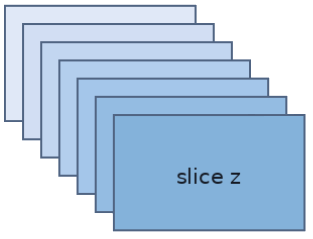
\includegraphics[scale=1.8]{figures/slices}
		\caption{\footnotesize{Structure of slices in the model.}}
	\end{figure}
	
	The neuronal signals used in this model should not be interpreted as the amplitude of individual biological action potentials. Biological spikes are essentially all-or-none events, while information can be represented by their frequency and temporal distribution. Instead, the continuous signal produced by a neuron in our model may be interpreted as an aggregate measure of neural activity over a short temporal interval, analogous to averaging the firing activity of biological neurons within a given sampling window. Thus, a large signal corresponds to intense activity during that interval, whereas a small or zero signal corresponds to weak or absent activity. This abstraction preserves a meaningful relation with biological firing-rate dynamics without requiring the explicit simulation of individual spikes, which would substantially increase the computational cost of the model.
	
	\subsection{Support Functions}
	
	To model how a gene $x = x_0 \ldots x_{p-1}$ generates a brain feature, we use functions of the form
	\begin{equation}
		\Phi(x) = \sum_{t=0}^{p-1} W(t) \cdot U(x_t),
	\label{Phi}
	\end{equation}
where $W(t)$ are the \emph{weights} of the function and $U(x_t)$ models how each digit of the gene acts on that feature. In this work, a few specific chosen $W$ and $U$ are used. However, in future work it is possible to test other families of functions or even allow these families to be genetically determined. What we need most from this model is for it to meet the following conditions:

	\begin{enumerate}
		\item The feature function is continuous over the real numbers.
		\item Genes that are nearby (according to the $L^1$ metric) usually exhibit similar features.
		\item In some cases, changing a single digit can have a significant impact.
	\end{enumerate}

The equations of this model can be combined with one another to obtain different distributions, depending on the objective at hand.	 Now we will discuss the specific functions chosen for our model.
	
	Whenever we want a brain parameter ranging in some interval, we will be changing the length $p$ of the gene and the base $\beta > 0$ in the equation
	\begin{equation}
		F_\beta(x) = \sum_{t=0}^{p-1} \sqrt{1 + t} \cdot \beta^{x_t}.
	\label{F}
	\end{equation}
	
	Weighting the individual values by $\sqrt{1 + t}$ is nothing special. The intention is to give positional weight to the gene digits. In particular, the positions of a gene are not required to have the same phenotypic influence. Since $\sqrt{1+t}$ increases with $t$, later digits have a larger contribution to the scalar parameters defined through this family. This positional hierarchy is intentional and was verified numerically to provide useful variation without making the mapping excessively irregular.
	
	\begin{figure}[H]
		\centering
		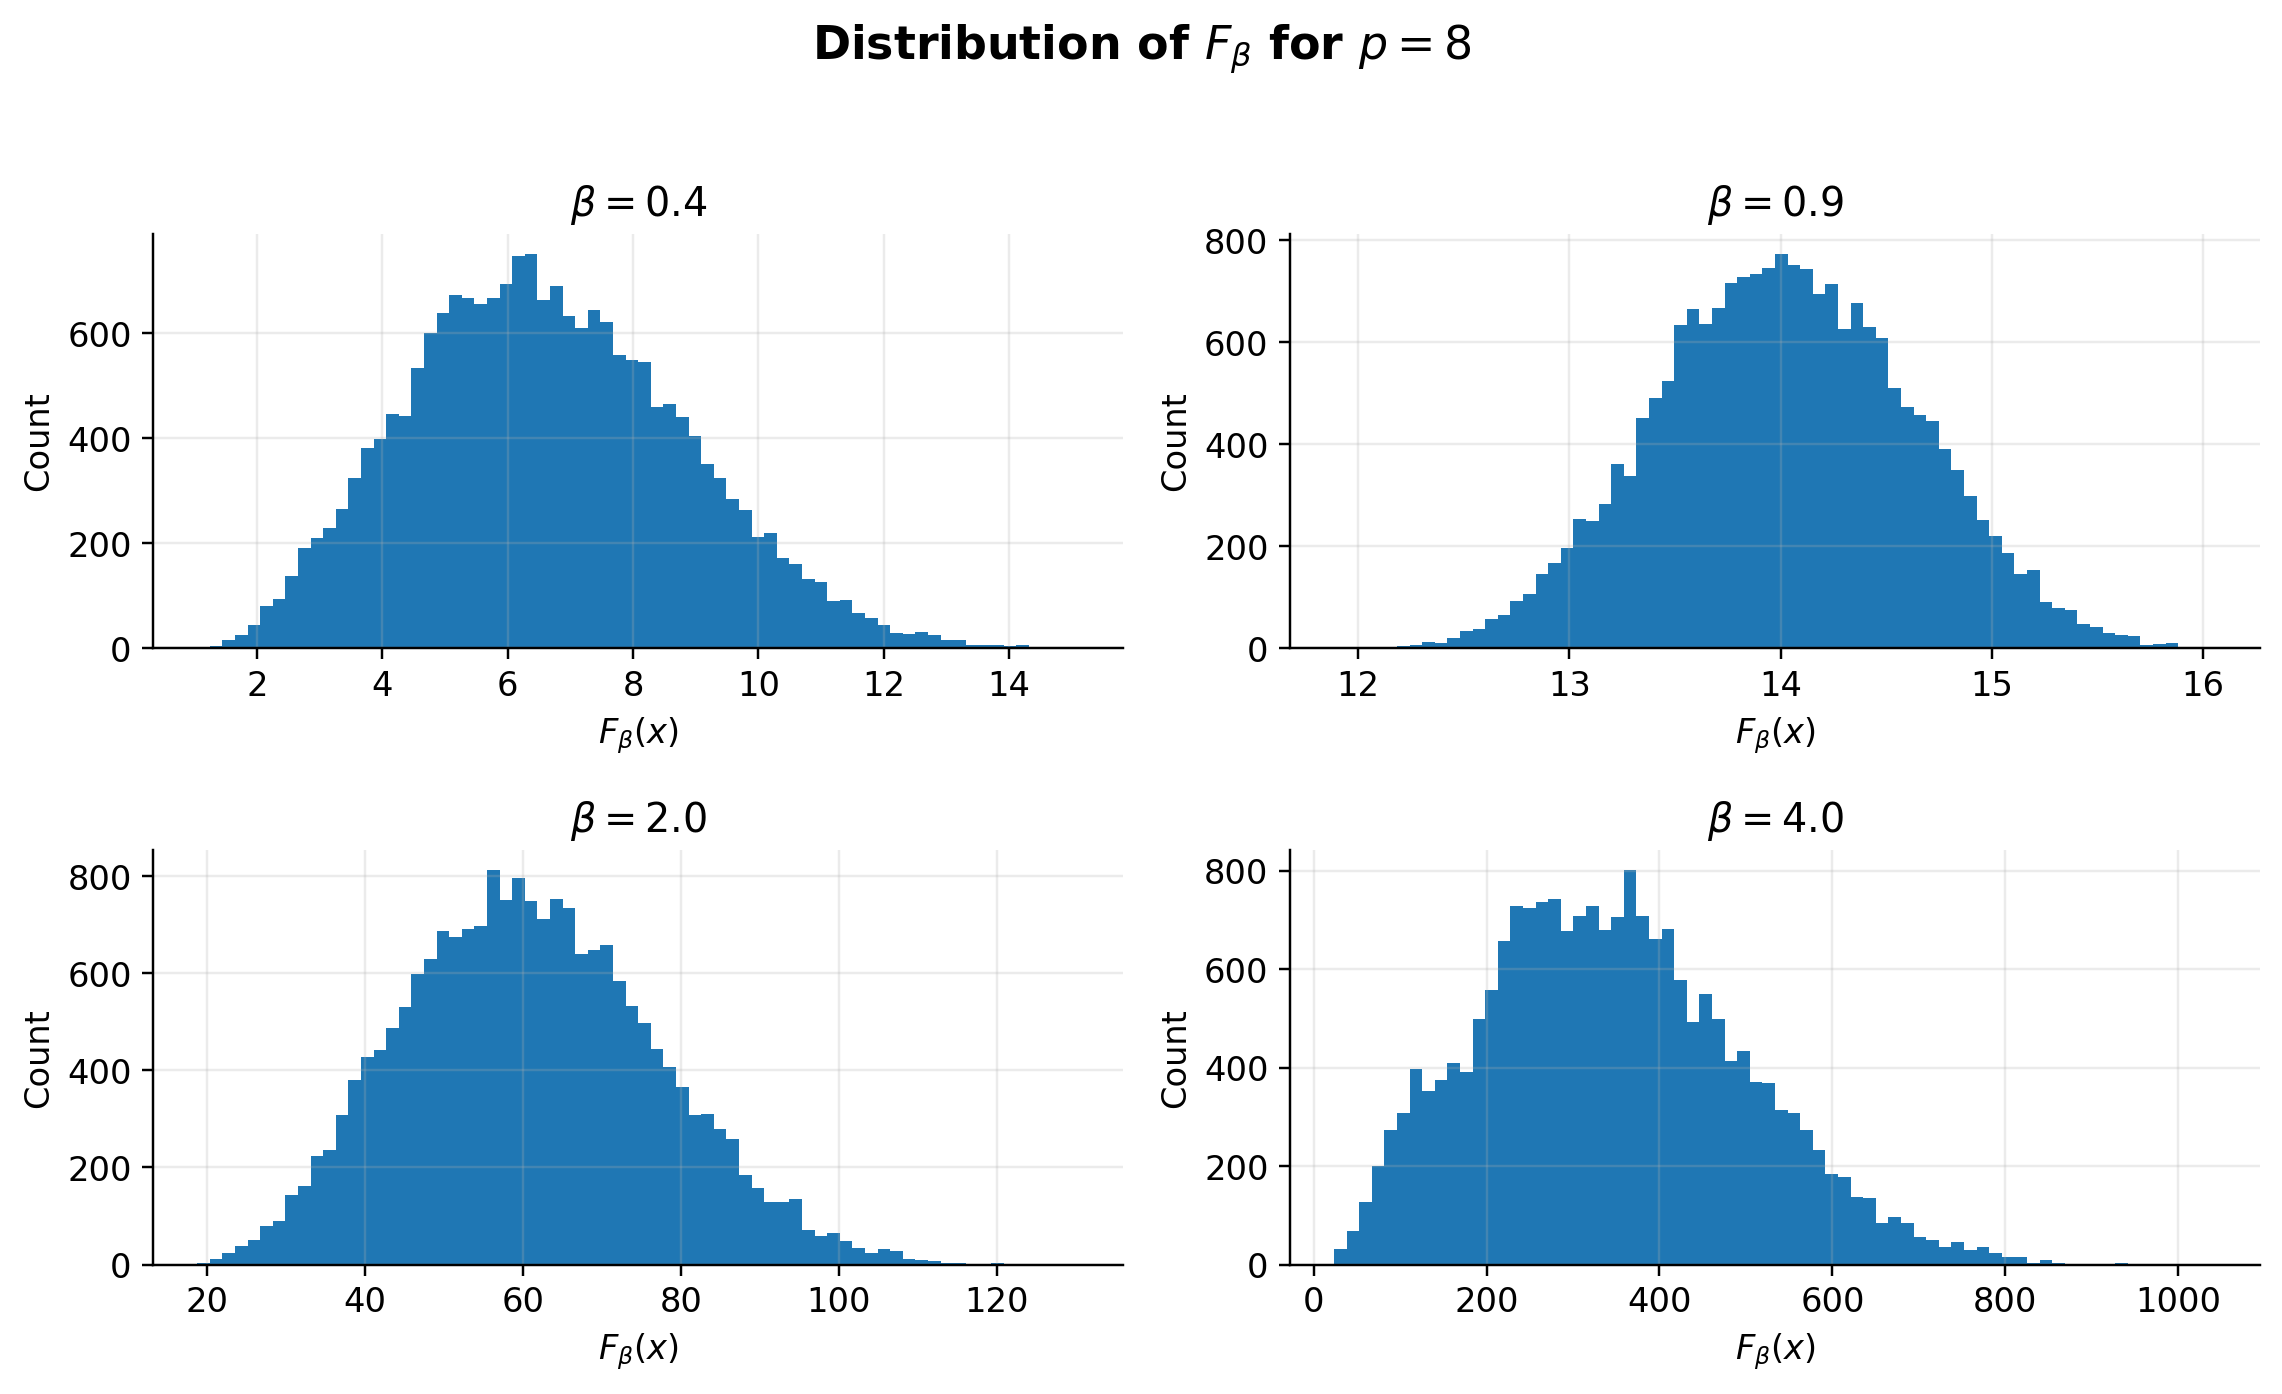
\includegraphics[width=0.95\linewidth,height=0.70\textheight,keepaspectratio]{generated_article_figures/F_distribution_p8.png}
		\caption{\footnotesize{Distribution of $F_\beta$ for $p=8$ fixed and $\beta \in \{ 0.4,\ 0.9,\ 2,\ 4 \}$. To generate the genes, each digit was drawn from the uniform distribution over $\{ 0, 1, 2, 3 \}$.}}
	\end{figure}
	
	\begin{figure}[H]
		\centering
		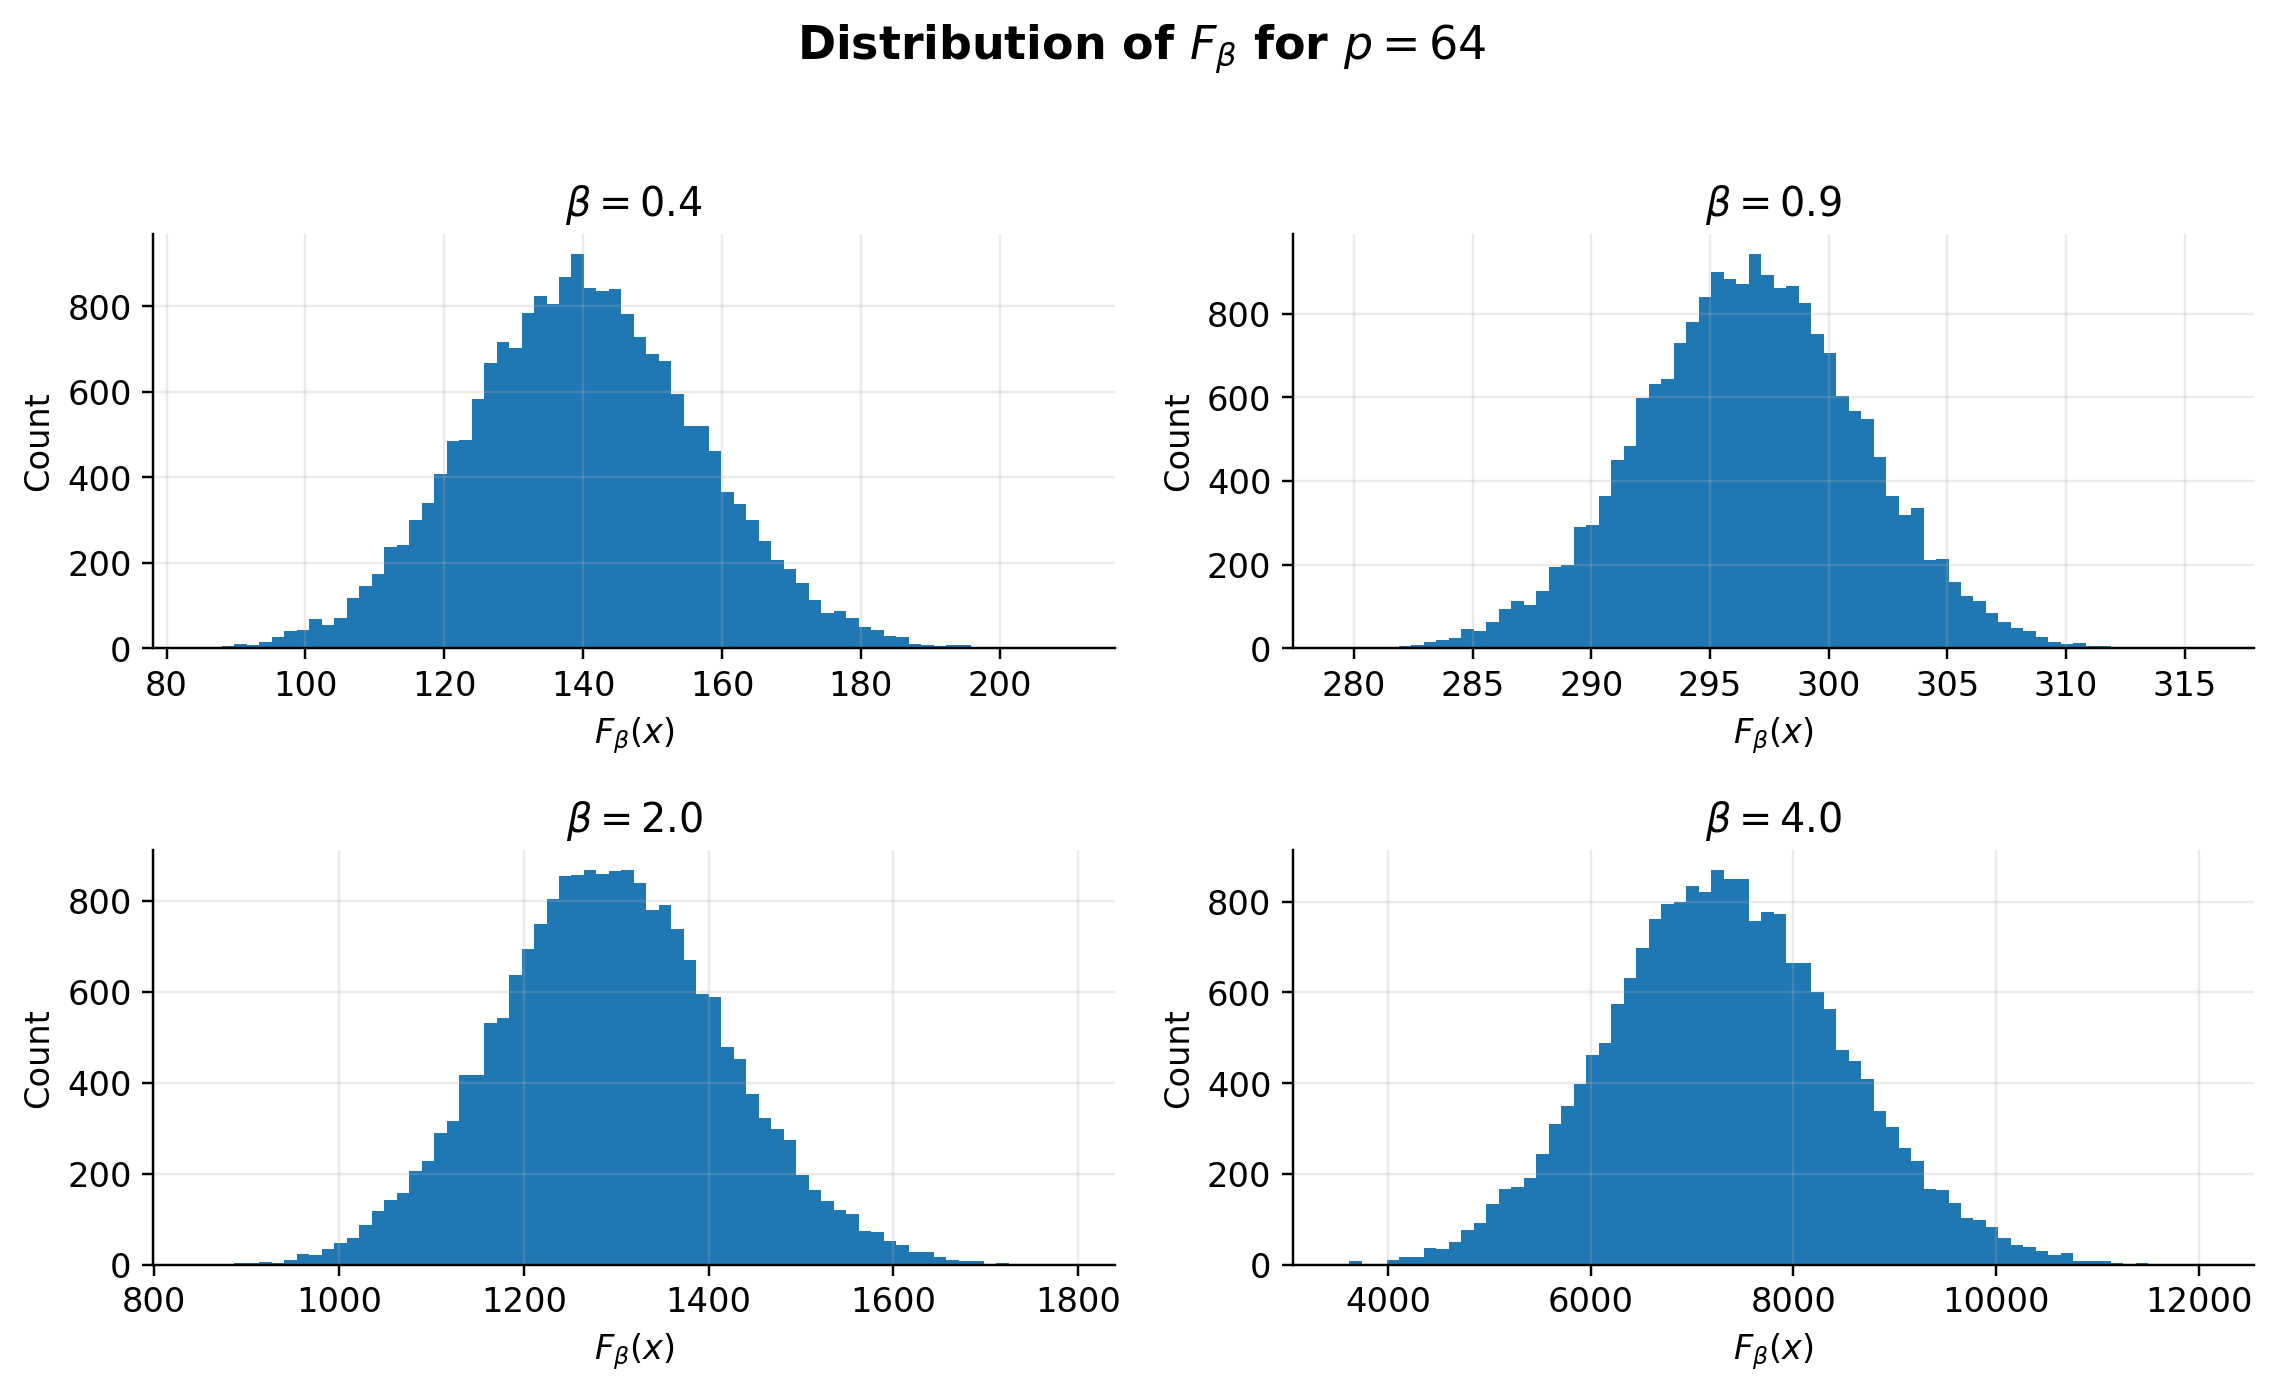
\includegraphics[width=0.95\linewidth,height=0.70\textheight,keepaspectratio]{generated_article_figures/F_distribution_p64.png}
		\caption{\footnotesize{Distribution of $F_\beta$ for $p=64$ fixed and $\beta \in \{ 0.4,\ 0.9,\ 2,\ 4 \}$. To generate the genes, each digit was drawn from the uniform distribution over $\{ 0, 1, 2, 3 \}$.}}
	\end{figure}
	
	We are also interested in knowing how nearby genes are mapped to nearby values by the defined mapping. For a fixed distance $\alpha \geq 0$ we have a level set $\{(x, y): d(x, y) = \alpha\}$. We may regard this level set as the set of genes with the same degree of similarity. The relative difference $\frac{|F_\beta(x) - F_\beta(y)|}{F_\beta(x)}$ in this level set can vary, with this variance increasing with the distance. Below, we show the distributions of these differences for each level set. 
	
	\begin{figure}[H]
		\centering
		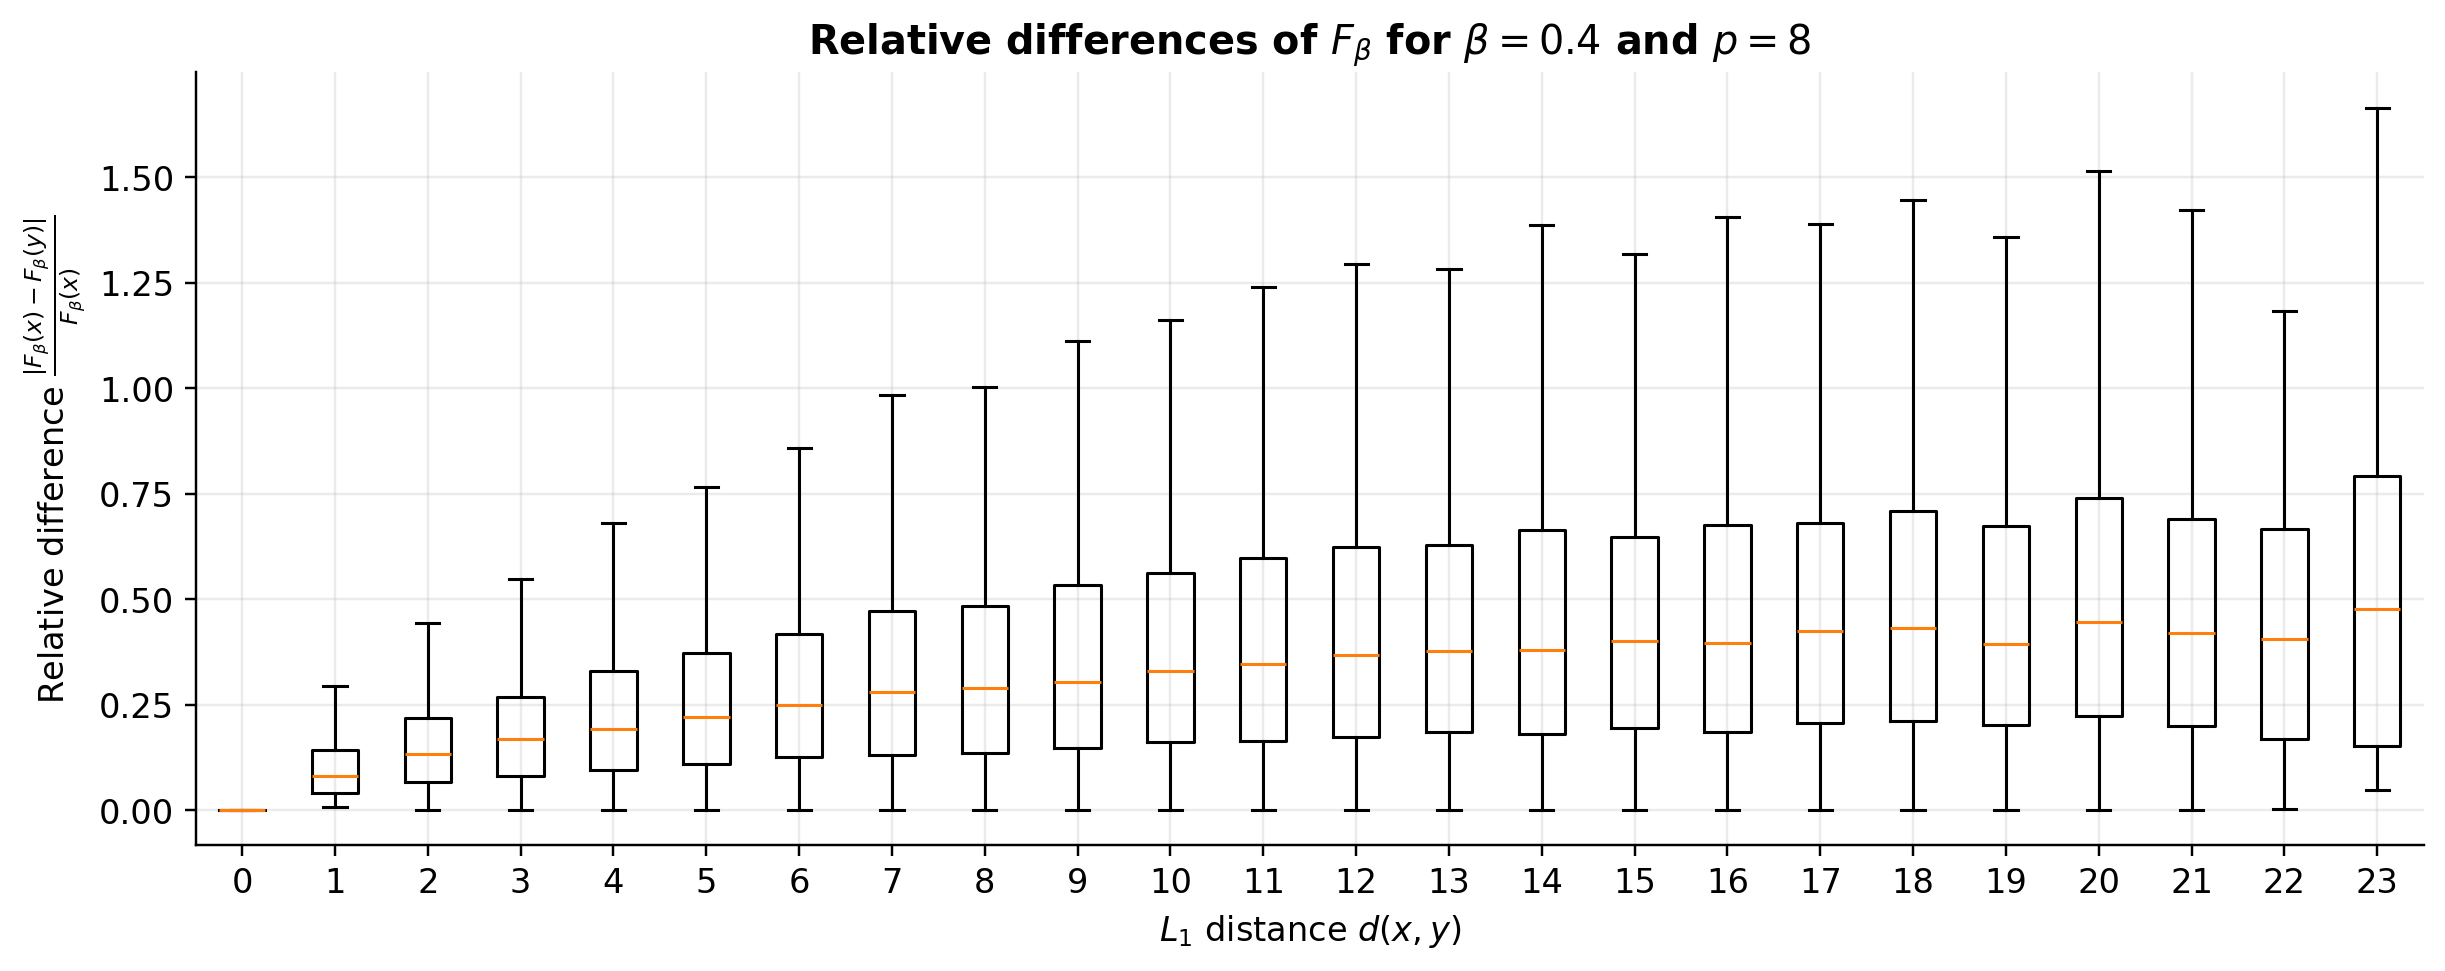
\includegraphics[width=0.93\linewidth,height=0.70\textheight,keepaspectratio]{generated_article_figures/F_relative_beta04_p8.png}
		\caption{\footnotesize{Box plot distribution of the relative differences $\frac{|F_\beta(x) - F_\beta(y)|}{F_\beta(x)}$ for $\beta = 0.4$ and $8$ digits per gene. To generate the genes, each digit was drawn from the uniform distribution over $\{ 0, 1, 2, 3 \}$.}}
	\end{figure}
	
	\begin{figure}[H]
		\centering
		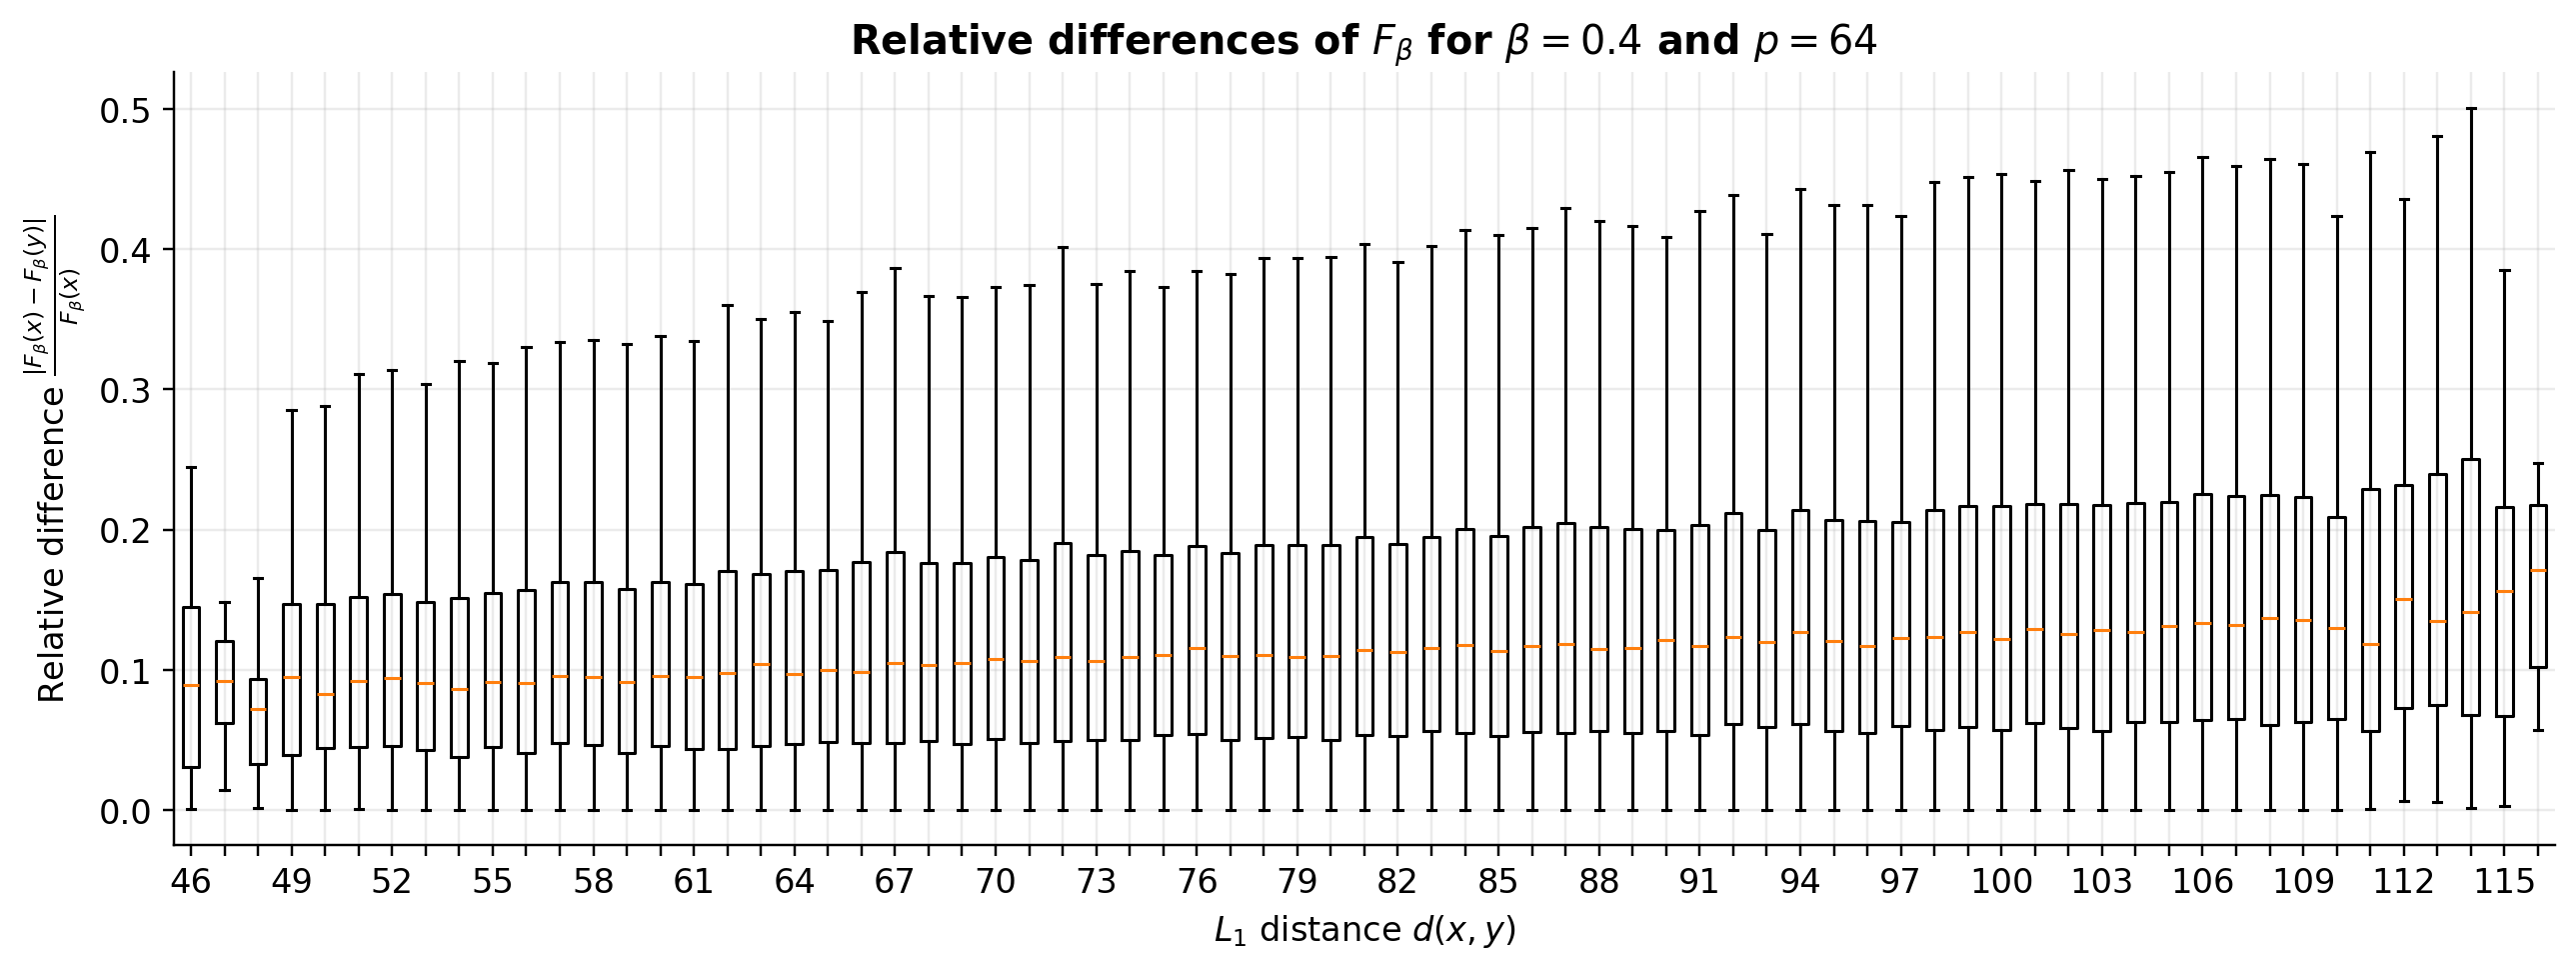
\includegraphics[width=0.93\linewidth,height=0.70\textheight,keepaspectratio]{generated_article_figures/F_relative_beta04_p64.png}
		\caption{\footnotesize{Box plot distribution of the relative differences $\frac{|F_\beta(x) - F_\beta(y)|}{F_\beta(x)}$ for $\beta = 0.4$ and $64$ digits per gene. The plot covers the entire range obtained from the samples. To generate the genes, each digit was drawn from the uniform distribution over $\{ 0, 1, 2, 3 \}$.}}
	\end{figure}
	
	\begin{figure}[H]
		\centering
		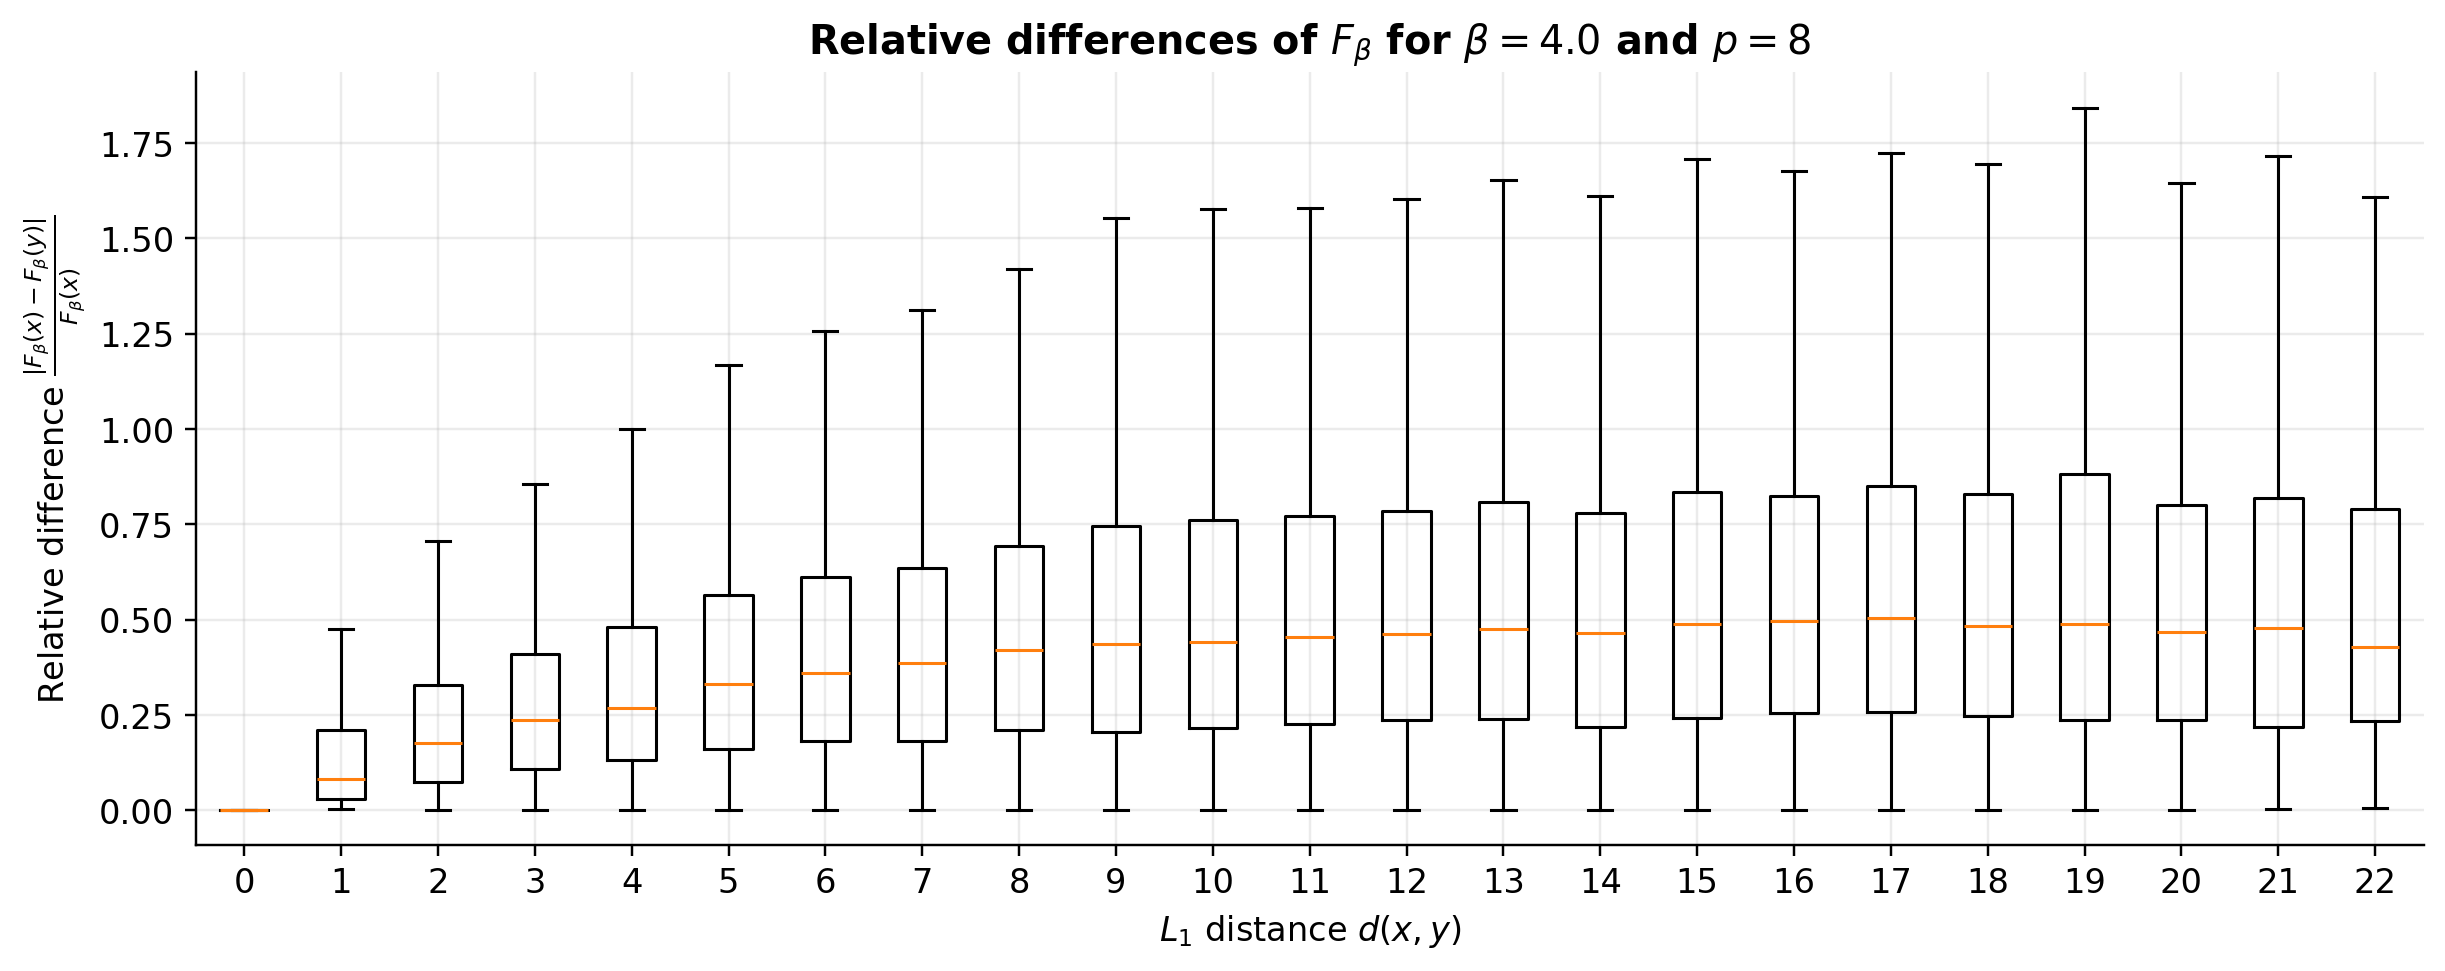
\includegraphics[width=0.93\linewidth,height=0.70\textheight,keepaspectratio]{generated_article_figures/F_relative_beta4_p8.png}
		\caption{\footnotesize{Box plot distribution of the relative differences $\frac{|F_\beta(x) - F_\beta(y)|}{F_\beta(x)}$ for $\beta = 4$ and $8$ digits per gene. To generate the genes, each digit was drawn from the uniform distribution over $\{ 0, 1, 2, 3 \}$.}}
	\end{figure}
	
	\begin{figure}[H]
		\centering
		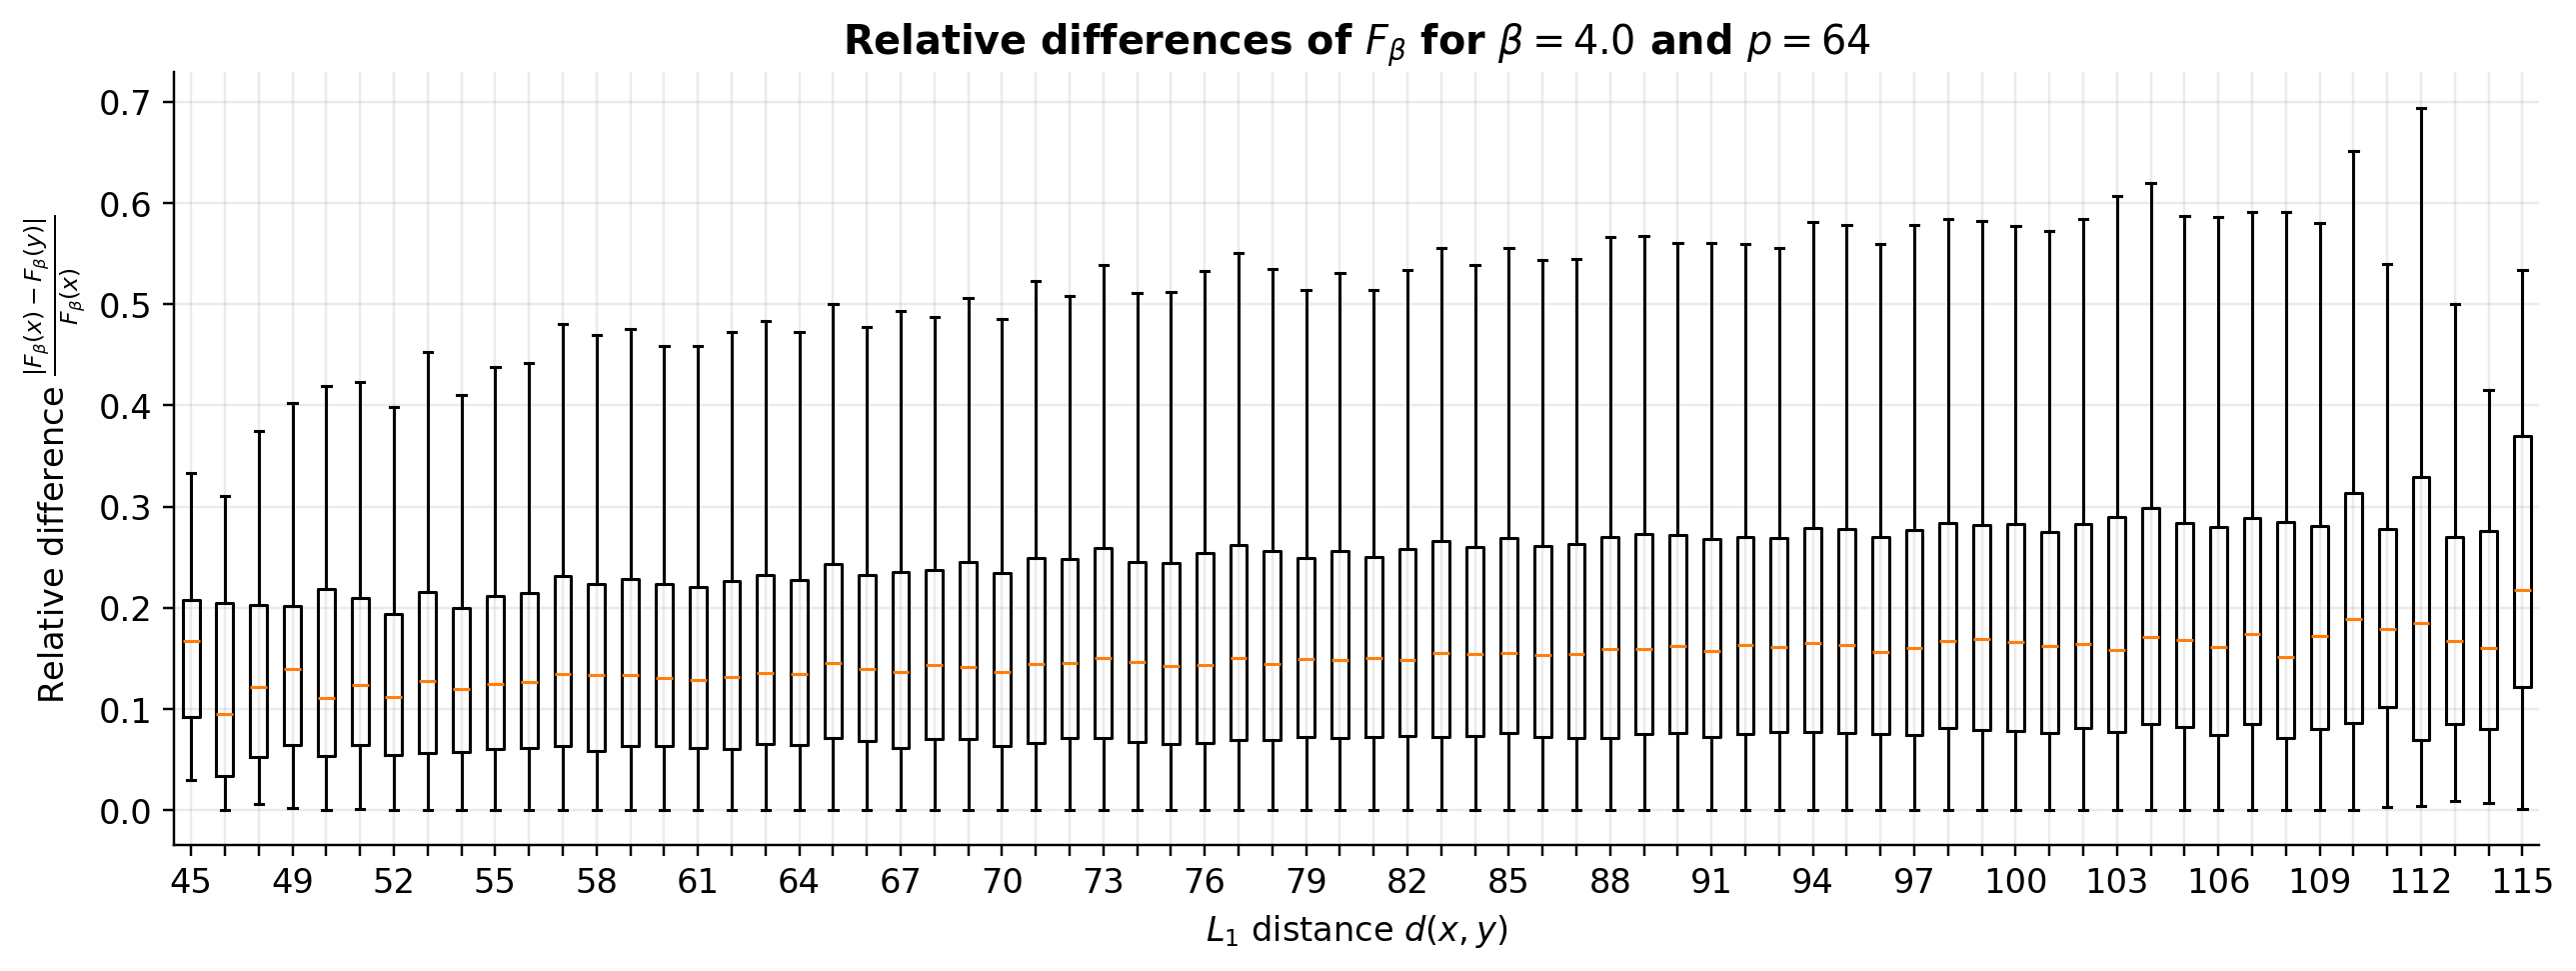
\includegraphics[width=0.93\linewidth,height=0.70\textheight,keepaspectratio]{generated_article_figures/F_relative_beta4_p64.png}
		\caption{\footnotesize{Box plot distribution of the relative differences $\frac{|F_\beta(x) - F_\beta(y)|}{F_\beta(x)}$ for $\beta = 4$ and $64$ digits per gene. The plot covers the entire range obtained from the samples. To generate the genes, each digit was drawn from the uniform distribution over $\{ 0, 1, 2, 3 \}$.}}
	\end{figure}
	
	Although increasing $p$ adds more terms to the sum, it also makes the total value more stable. The expected value of $F_\beta(x)$ grows approximately as $p^{3/2}$, while its typical fluctuations grow only as $p$. As a result, the relative variability scales roughly as $1/\sqrt{p}$. Therefore, larger values of $p$ tend to produce smaller relative differences $|F_\beta(x)-F_\beta(y)|/F_\beta(x)$, even though the absolute differences may increase.
	
	As explained, equation~\ref{F} may be regarded as a weighted sum. Another type of weighted sum is given by equation
	\begin{equation}
		G_{\delta_1, \delta_2}(x) = \sum_{t=0}^{p-1} \sin(1 + t) \sin(1 + x_t)^{\delta_1} \cos(1 + x_t)^{\delta_2}.	
	\label{G}
	\end{equation}
	
	The weights in this equation are the terms $\sin(1 + t)$. Furthermore, in this definition we have that $\delta_i \in \{ 0, 1 \}$, with $\delta_1 + \delta_2 > 0$. Each choice gives a different kind of weighted sum. 
	
	\begin{figure}[H]
		\centering
		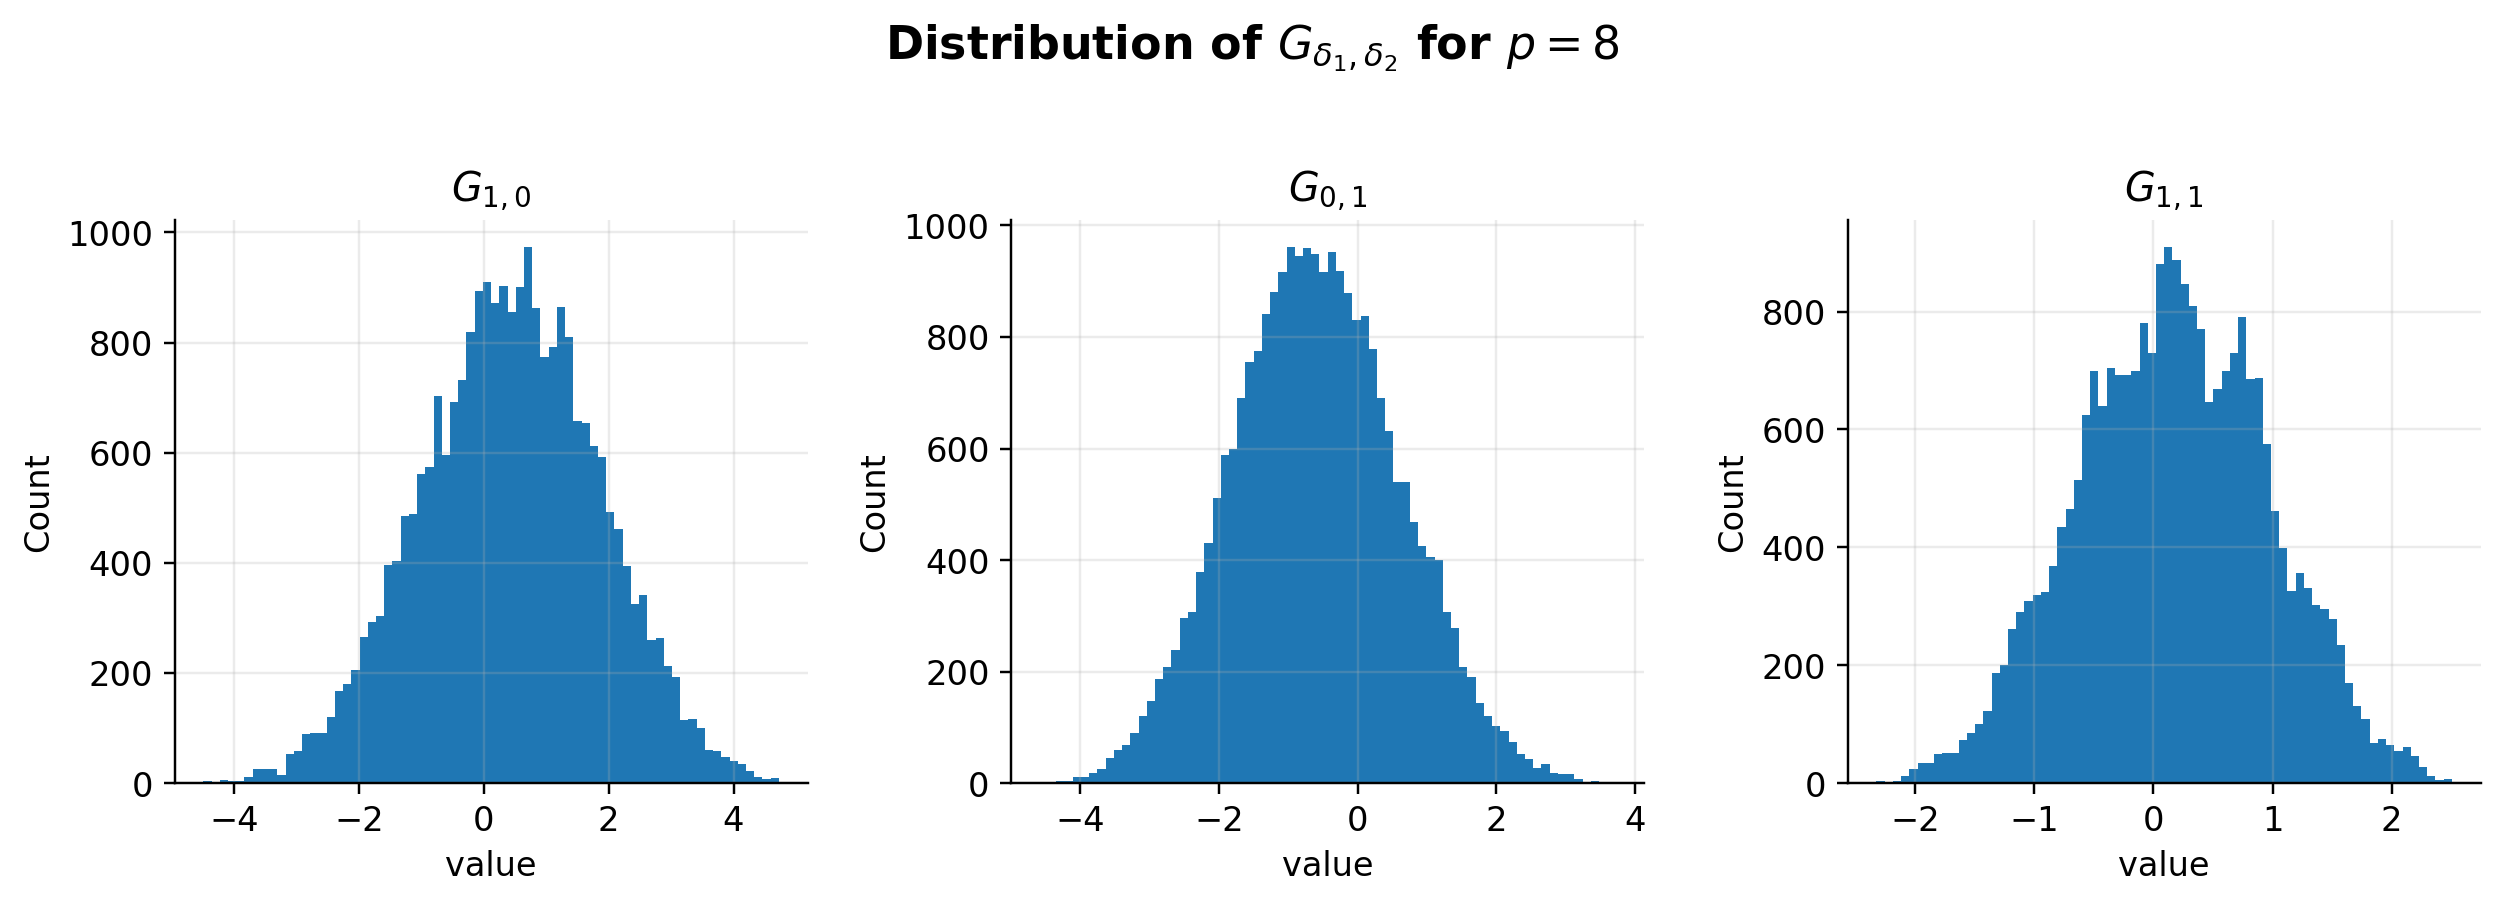
\includegraphics[width=0.93\linewidth,height=0.70\textheight,keepaspectratio]{generated_article_figures/G_distribution_p8.png}
		\caption{\footnotesize{Distribution of $G_{\delta_1, \delta_2}$ for $8$ digits per gene. To generate the genes, each digit was drawn from the uniform distribution over $\{ 0, 1, 2, 3 \}$.}}
	\end{figure}
	
	\begin{figure}[H]
		\centering
		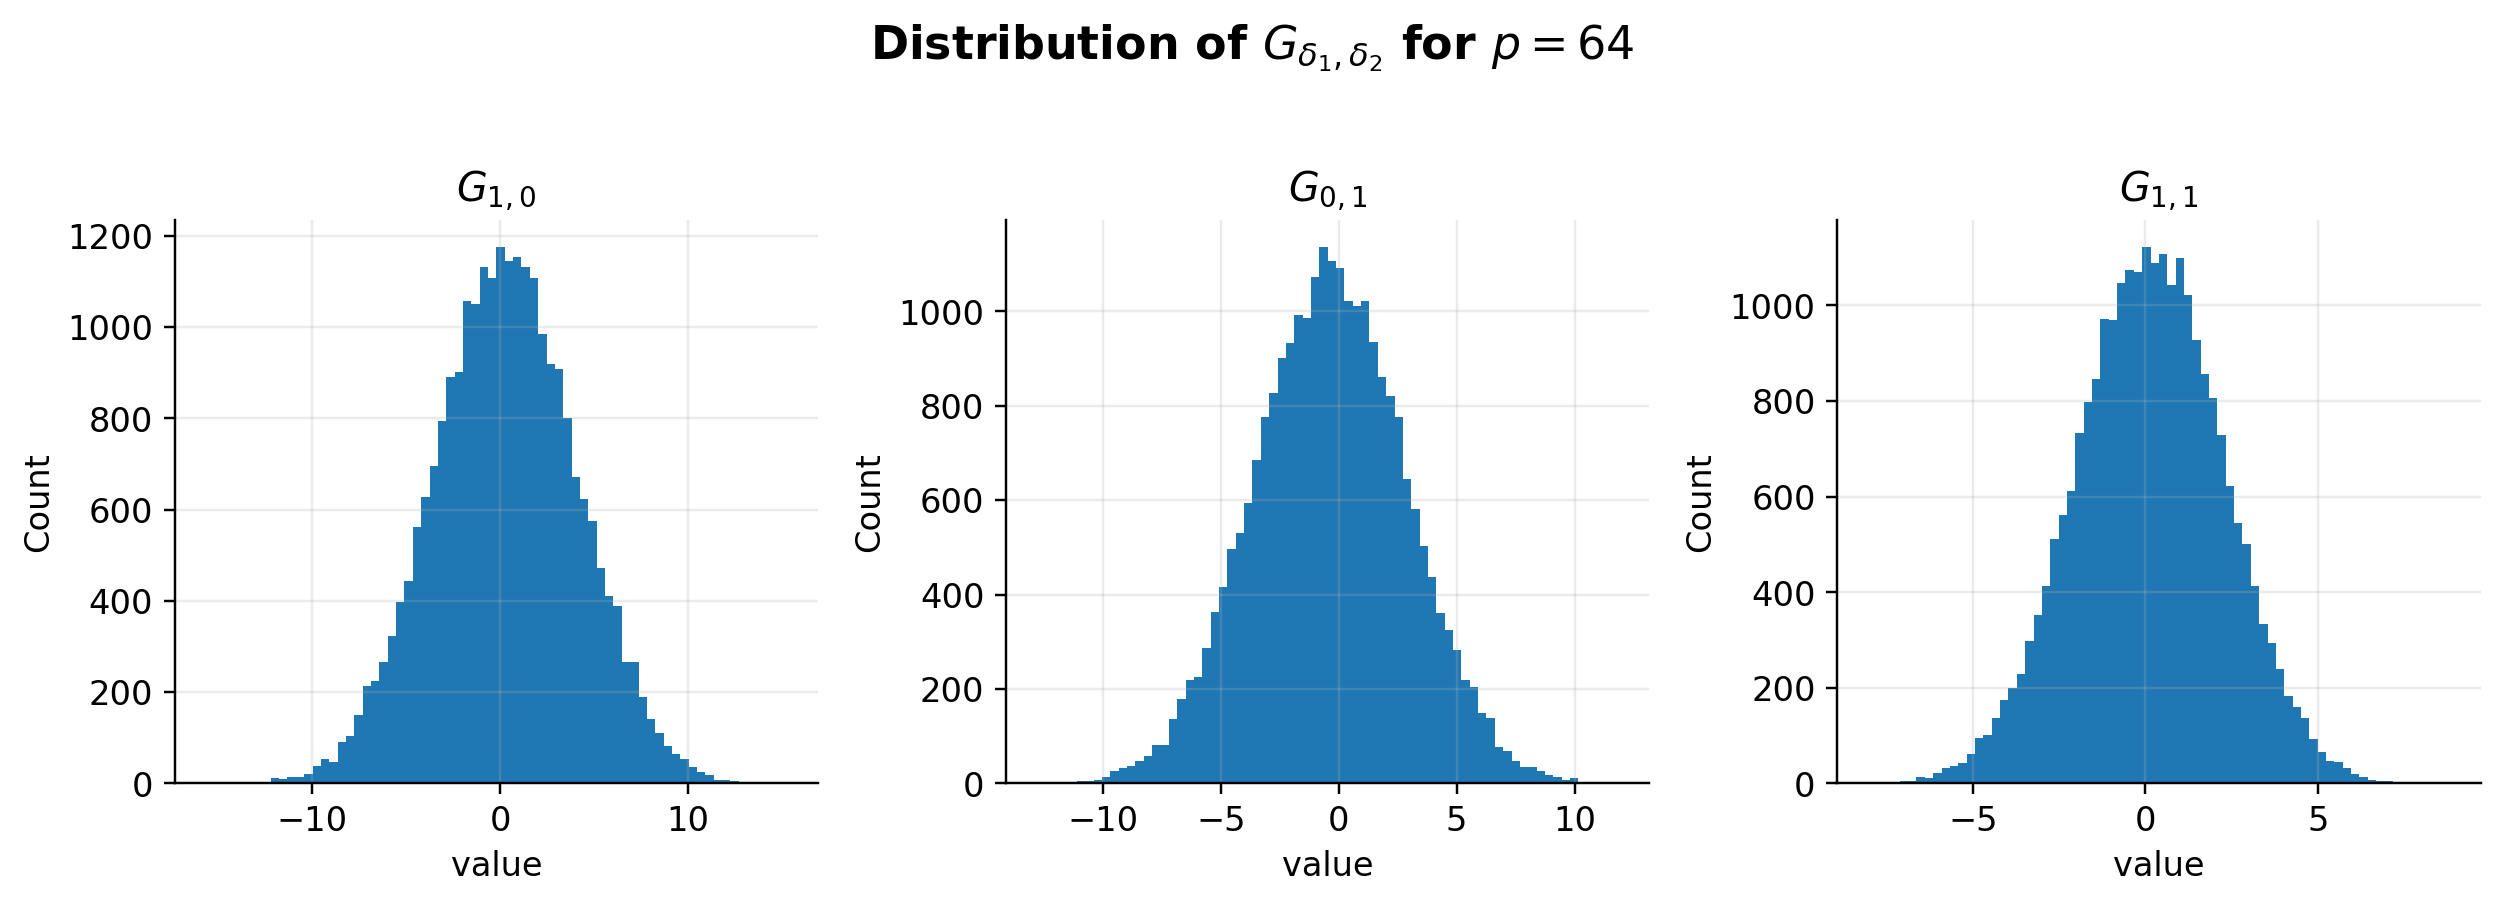
\includegraphics[width=0.93\linewidth,height=0.70\textheight,keepaspectratio]{generated_article_figures/G_distribution_p64.png}
		\caption{\footnotesize{Distribution of $G_{\delta_1, \delta_2}$ for $64$ digits per gene. To generate the genes, each digit was drawn from the uniform distribution over $\{ 0, 1, 2, 3 \}$.}}
	\end{figure}
	
	Let $(I,J,K)$ denote the dimensions of the brain and $(i,j,k)$ an integer lattice position, with $0\leq i<I$, $0\leq j<J$, and $0\leq k<K$. The spatial coordinates used by the genetic field are

	$$a=\frac{i}{L},\qquad b=\frac{j}{L},\qquad c=\frac{k}{L},\qquad L=16.$$

	The length $L$ is a fixed external spatial scale (in lattice steps), shared by the three axes and independent of the brain dimensions. Unlike normalization by $I-1$, $J-1$, and $K-1$, this choice keeps the local spatial sampling scale unchanged as the brain grows. In particular, the same genome produces exactly the same mathematical field value at any lattice coordinate contained in two differently sized brains. Increasing the dimensions extends the sampled domain instead of refining a fixed unit cube, this is the intended spatial ``zoom-out'' behavior. The precise scale $L=16$ is a modeling choice and is not inferred from biological data.

	Let the gene be	$x = x_0 \ldots x_{p-1}$ and assume that $p=n^3$. The correspondence between the gene index and the spatial mode is

	$$t=q+ns+n^2r.$$

	Each digit of the gene is mapped to a scalar coefficient in $[-1,1]$ according to

	$$\alpha(x_t)=\frac{2x_t}{3}-1.$$

	Therefore,

	$$0\mapsto-1,\qquad 1\mapsto-\frac{1}{3},\qquad 2\mapsto\frac{1}{3},\qquad 3\mapsto1.$$

	To avoid a common period imposed by integer spatial frequencies, we use the fixed mode frequencies

	$$\omega_r=\sqrt{r+1},\qquad r=0,\ldots,n-1.$$

	The scalar field is defined by

	\begin{equation}
	A_{i,j,k}(x)=\tanh\left(\frac{1}{\sqrt{p}}\sum_{r=0}^{n-1}\sum_{s=0}^{n-1}\sum_{q=0}^{n-1}\alpha\!\left(x_{q+ns+n^2r}\right)\cos(\pi\omega_r a)\cos(\pi\omega_s b)\cos(\pi\omega_q c)\right).
	\label{A}
	\end{equation}

	For the implemented 64-digit spatial genes, $n=4$ and the frequencies are $1,\sqrt{2},\sqrt{3},2$. Their irrational ratios prevent a common nonzero spatial period for a generic field in which the corresponding modes remain present. They do not rule out special degenerate combinations of coefficients, nor do they preclude arbitrarily close approximate recurrences: a finite sum of incommensurate trigonometric modes is almost periodic. The cosine basis still has reflection symmetry about the coordinate origin. Accordingly, the formulation permits spatial variation over larger brains without promising an unlimited number of distinct regions or automatic functional specialization.
	
	The factor $1/\sqrt{p}$ keeps the typical scale of the field approximately stable as the number of modes changes. Since the coefficients $\alpha(x_t)$ are centered around zero, the unnormalized sum exhibits cancellations and its typical magnitude grows on the order of $\sqrt{p}$ rather than $p$.
	
	The correspondence $t=q+ns+n^2r$ assigns each gene position to a unique spatial mode. Any mixing of spatial positions is therefore produced by the field itself rather than by an index collision. Gene positions are not intended to be phenotypically equivalent: their influence depends on the spatial mode $(q,s,r)$ rather than on an explicit increasing weight. Lower-frequency modes vary more broadly in space, whereas higher-frequency modes introduce finer variation. In contrast with the preceding integer-frequency formulation, $t=0$ is no longer a constant mode: it is the lowest-frequency product $\cos(\pi a)\cos(\pi b)\cos(\pi c)$. Every mode is position dependent, although all cosine factors equal one at the origin. Consequently, changes in a single digit can affect different regions differently, and the baseline $A_{0,0,0}(x)$ remains well defined for the polarity rule below. Changing the dimensions can also change the distribution of excitation and inhibition, since a larger domain samples additional values relative to this fixed baseline.

	Figures~\ref{fig:spatial_A_slices}--\ref{fig:spatial_A_mutations} illustrate how a 64-digit connections gene generates spatial structure. In the slice heatmaps, $k$ is fixed within each panel while $i$ and $j$ vary. The color limits remain fixed across slices and across genes, so color changes are directly comparable rather than rescaled panel by panel. These are illustrative realizations, not estimates of the distribution of all possible genomes.

	\begin{figure}[H]
		\centering
		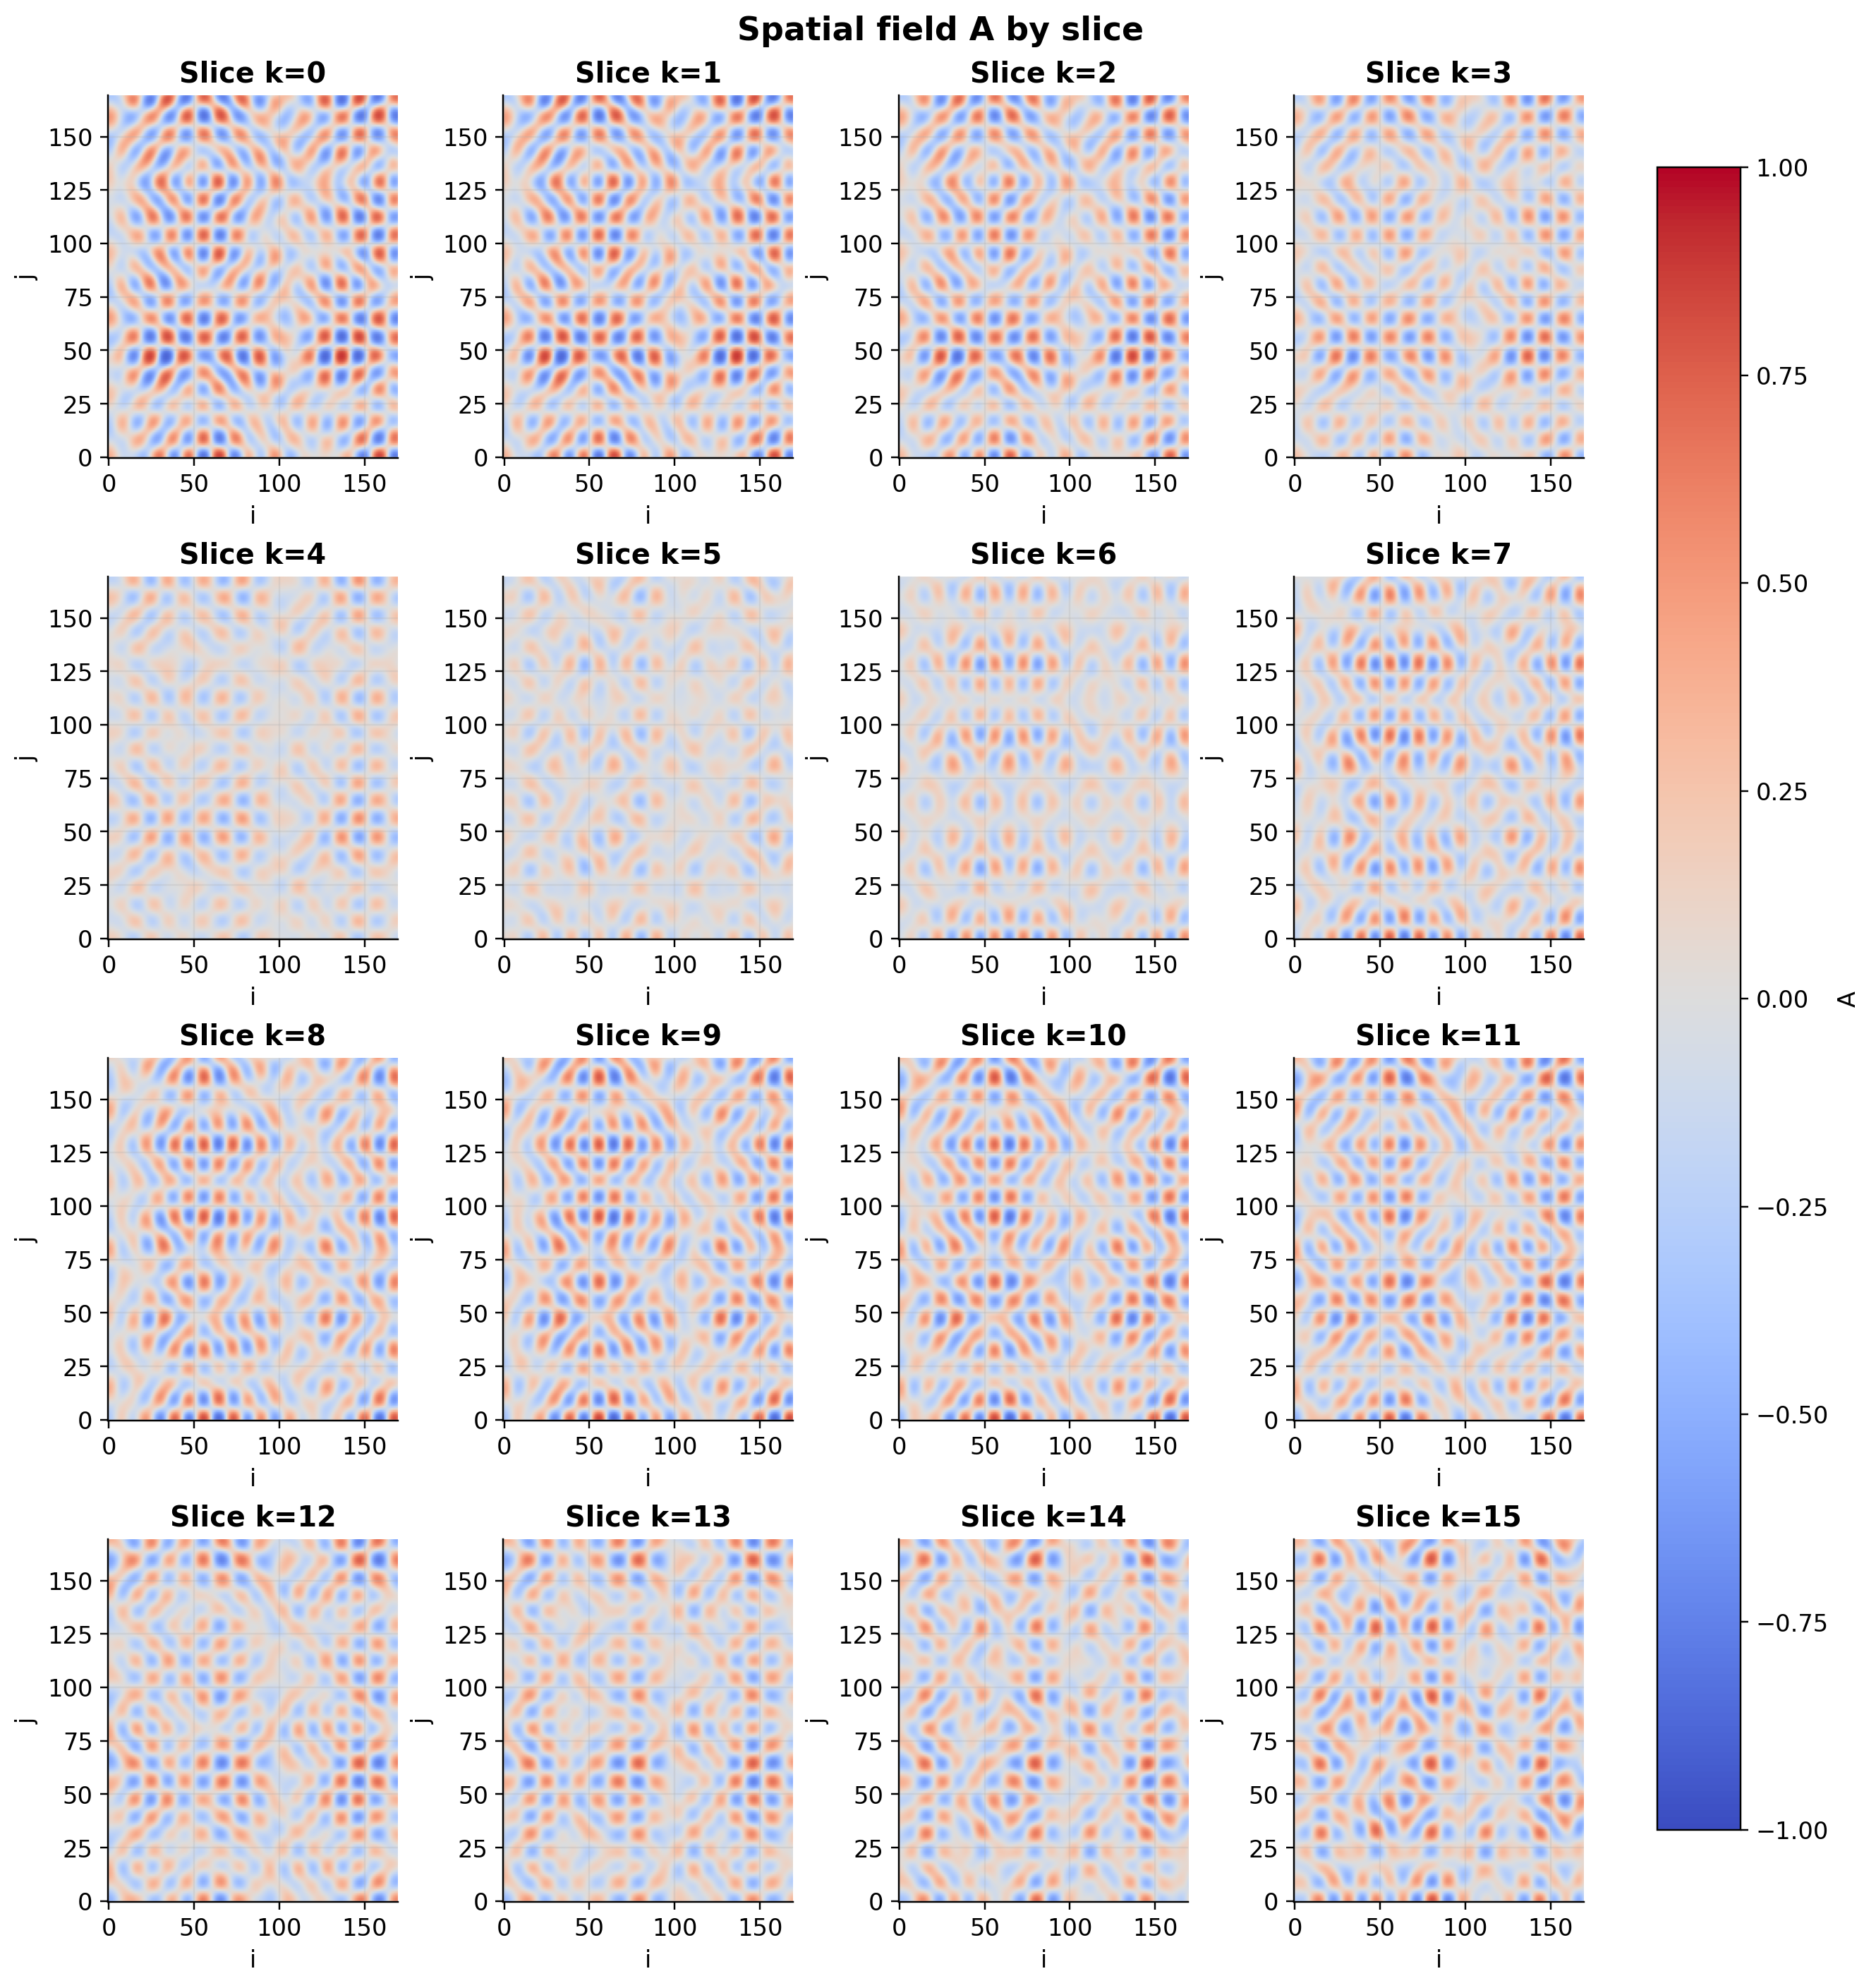
\includegraphics[width=0.98\linewidth,height=0.68\textheight,keepaspectratio]{generated_article_figures/extra_A_heatmaps.png}
		\caption{\footnotesize{Spatial field $A$ generated by one 64-digit connections gene in a brain with dimensions $(I,J,K)=(170,170,16)$. Each panel shows the values $A_{i,j,k}(x)$ at a different fixed $k$, with the same color scale $[-1,1]$ for all slices.}}
		\label{fig:spatial_A_slices}
	\end{figure}

	\begin{figure}[H]
		\centering
		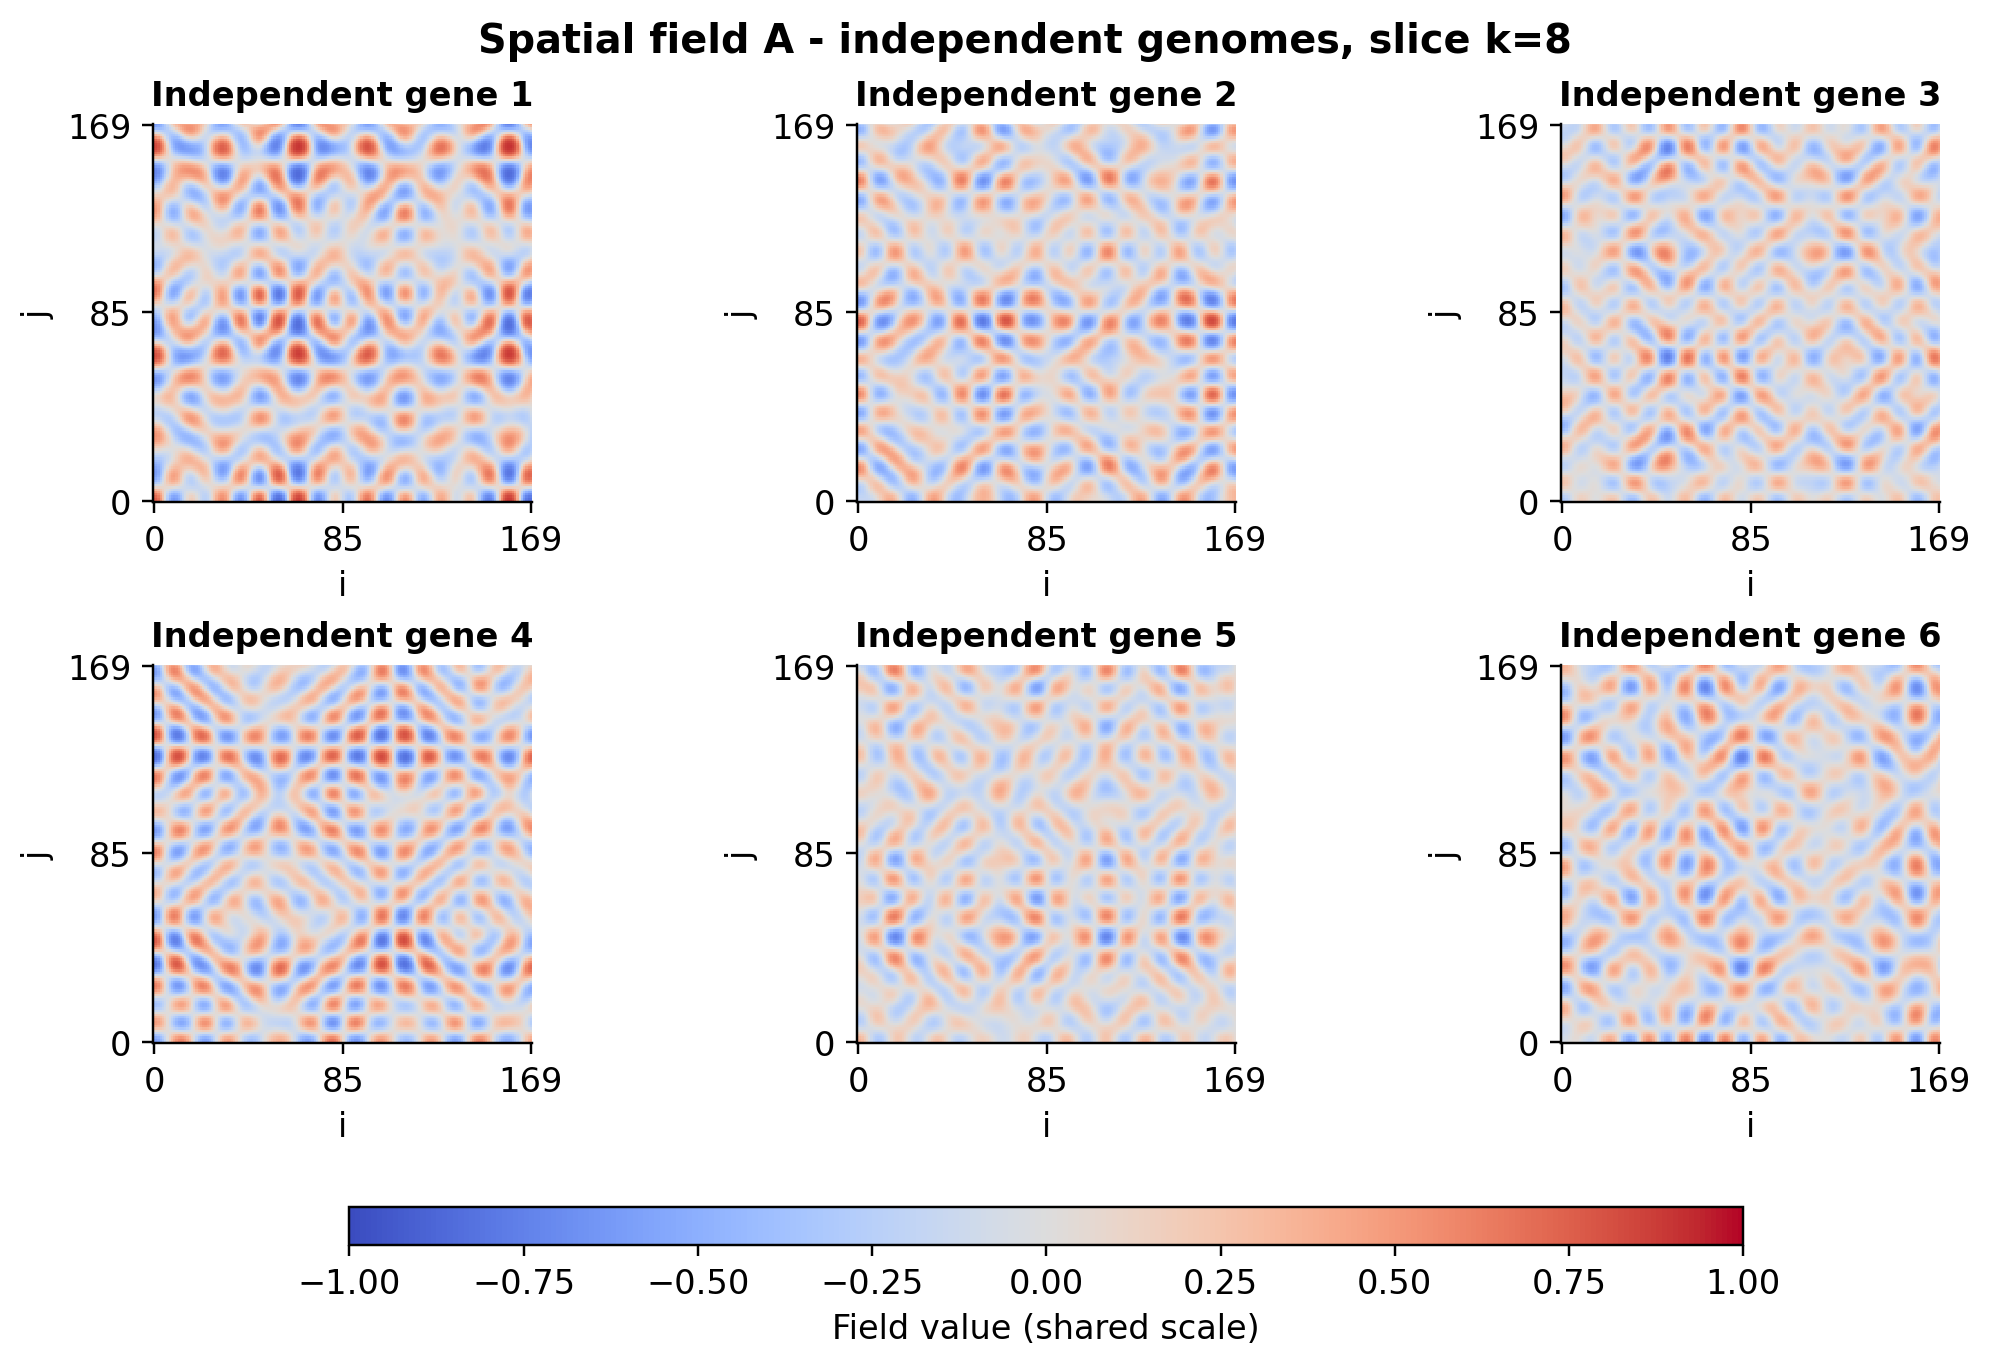
\includegraphics[width=0.98\linewidth,height=0.63\textheight,keepaspectratio]{generated_article_figures/extra_A_independent_genes_fixed_slice.png}
		\caption{\footnotesize{Comparison of the spatial field $A_{i,j,8}(x)$ for six independently sampled 64-digit connections genes, evaluated on the same $(170,170,16)$ tensor. The slice index and color scale $[-1,1]$ are held fixed, only the gene changes.}}
		\label{fig:spatial_A_genes}
	\end{figure}

	\begin{figure}[H]
		\centering
		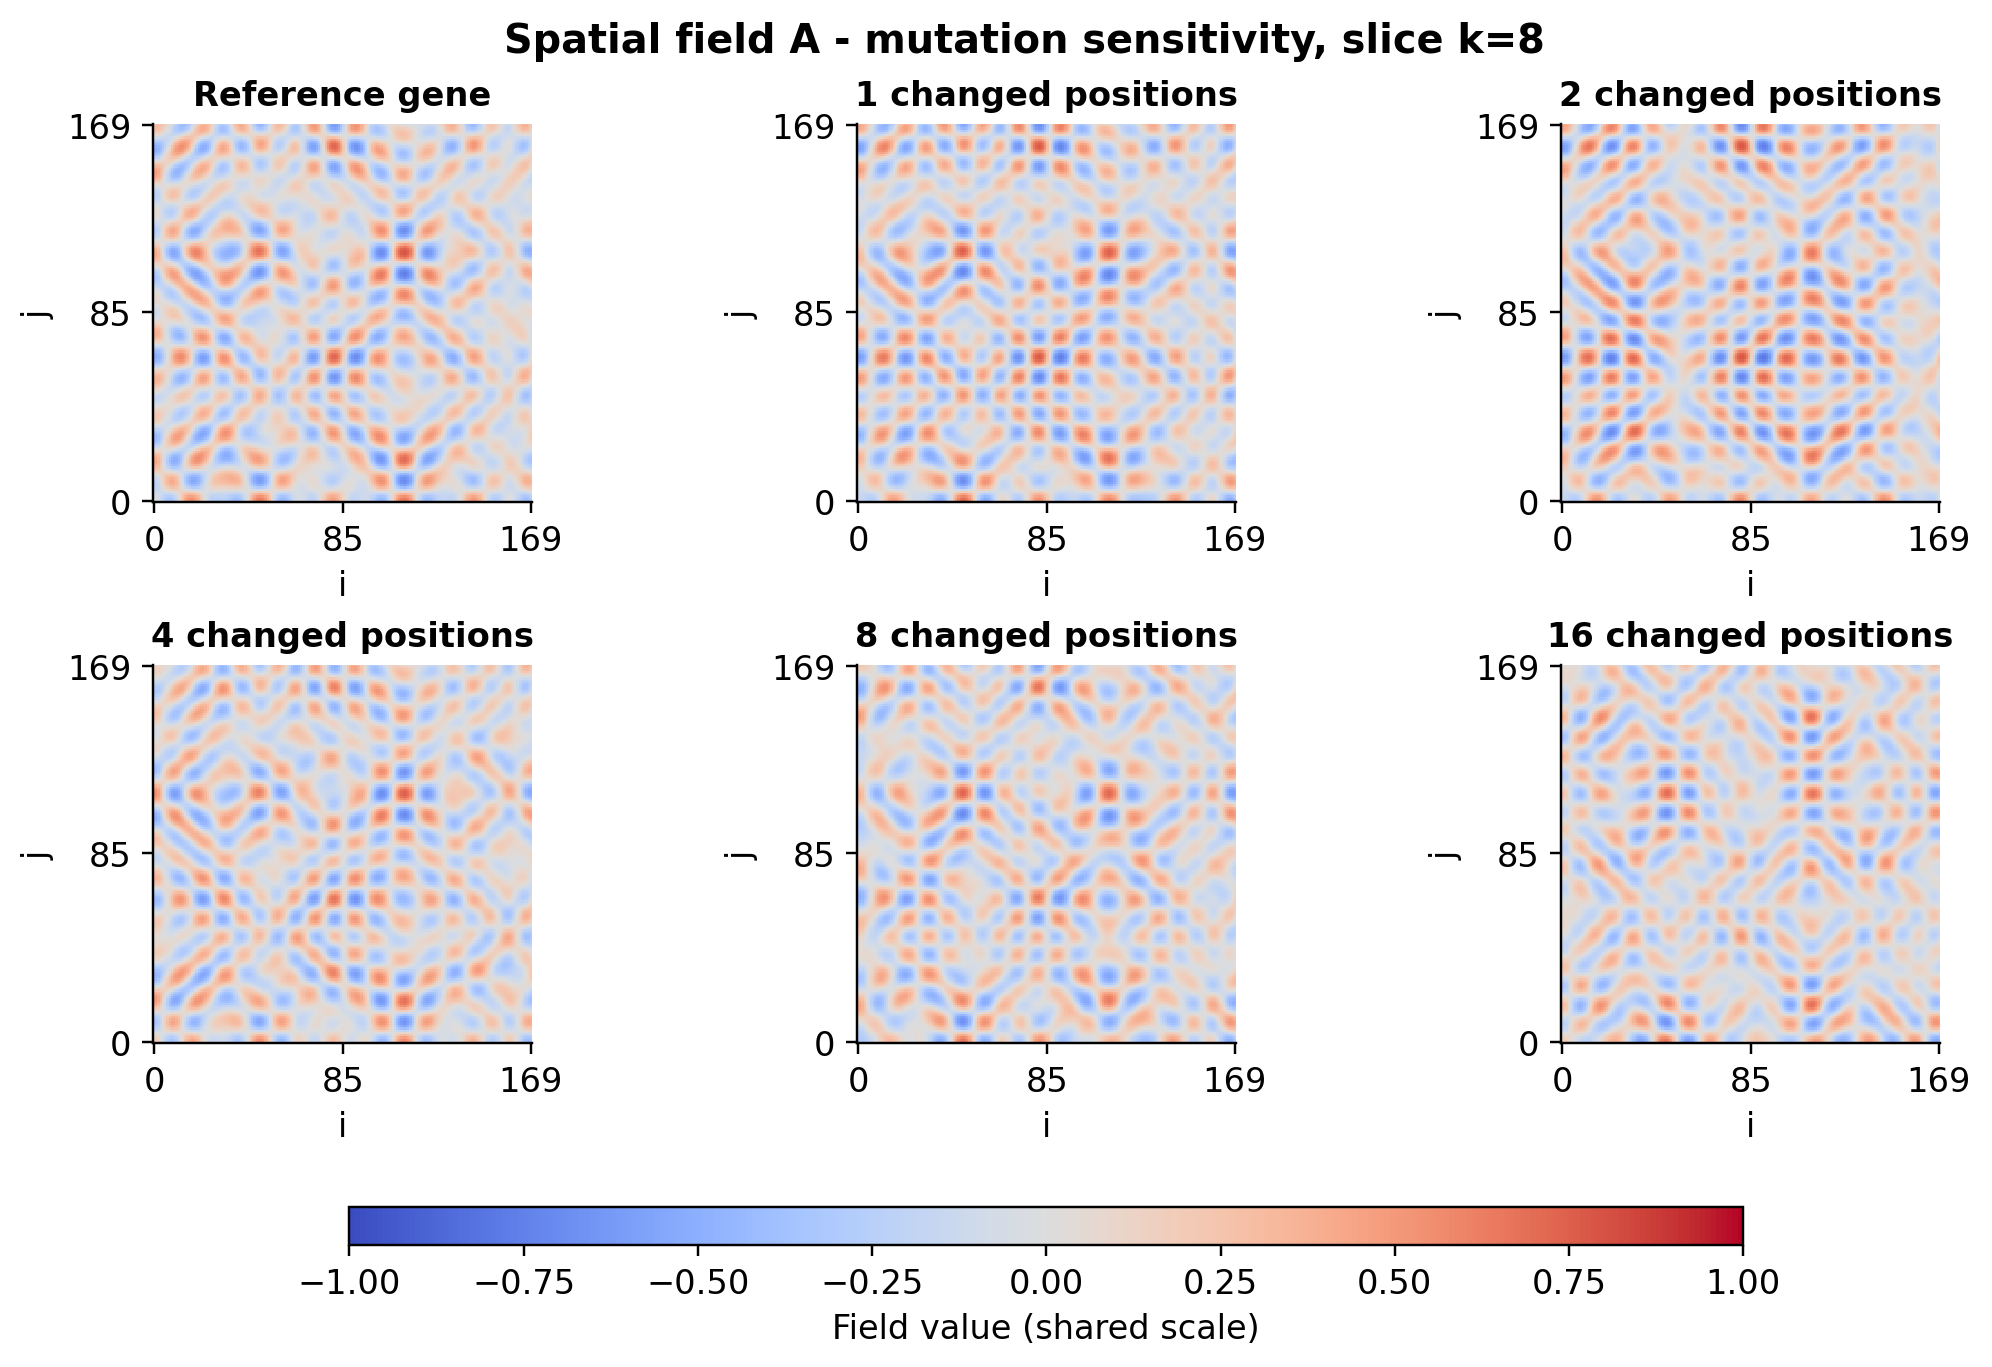
\includegraphics[width=0.98\linewidth,height=0.63\textheight,keepaspectratio]{generated_article_figures/extra_A_mutations_fixed_slice.png}
		\caption{\footnotesize{Response of the field $A_{i,j,8}(x)$ to genetic perturbations. Starting from a reference 64-digit gene, exactly $1$, $2$, $4$, $8$, or $16$ distinct digit positions are replaced by different values. Every panel uses the same slice and color scale $[-1,1]$.}}
		\label{fig:spatial_A_mutations}
	\end{figure}

	The first comparison isolates differences between independent genomes, whereas the second isolates changes relative to a common reference. Neighboring slices may share spatial motifs even when the field is not merely multiplied by a slice-dependent scalar, the figures alone do not quantify that distinction.
	
	Another useful auxiliary is the following.
	
	\begin{equation}
		H_{i,j,k}(u, v, w, x) = \sin\left( \frac{3\pi}{8} + \frac{4}{C} \sum_{t=0}^{p-1} \sqrt{1 + t} \cdot \Big( \sin \big( A_{i, j, k}(x) \cdot U(x_t) \big) + \cos \big( A_{u, v, w}(x) \cdot U(x_t) \big) \Big) \right) ,
	\label{H}
	\end{equation}
	
where $$C = \sum_{t=0}^{p-1} \sqrt{1 + t}.$$ 
			
	
	Unlike the spatial-mode expansion defining $A$, the same two values $A_{i,j,k}(x)$ and $A_{u,v,w}(x)$ are reused in every term of this sum. The normalization factor $4/C$, with $C$ equal to the total positional weight, controls the scale of the weighted sum as the gene length changes. The outer shift is $3\pi/8$. 
	
	This function is used when it is necessary to relate two distinct neurons through some value.

	Figures~\ref{fig:affinity_H_slices}--\ref{fig:affinity_H_mutations} show the spatial variation and genetic sensitivity of $H$ before the initial connection-search restrictions are applied. In all $H$ illustrations, the source coordinate is held fixed at $(85,85,8)$ while the candidate target position varies. For comparisons between genes, both $A$ and the coefficients of $H$ are recalculated from the same connections gene in each panel.

	\begin{figure}[H]
		\centering
		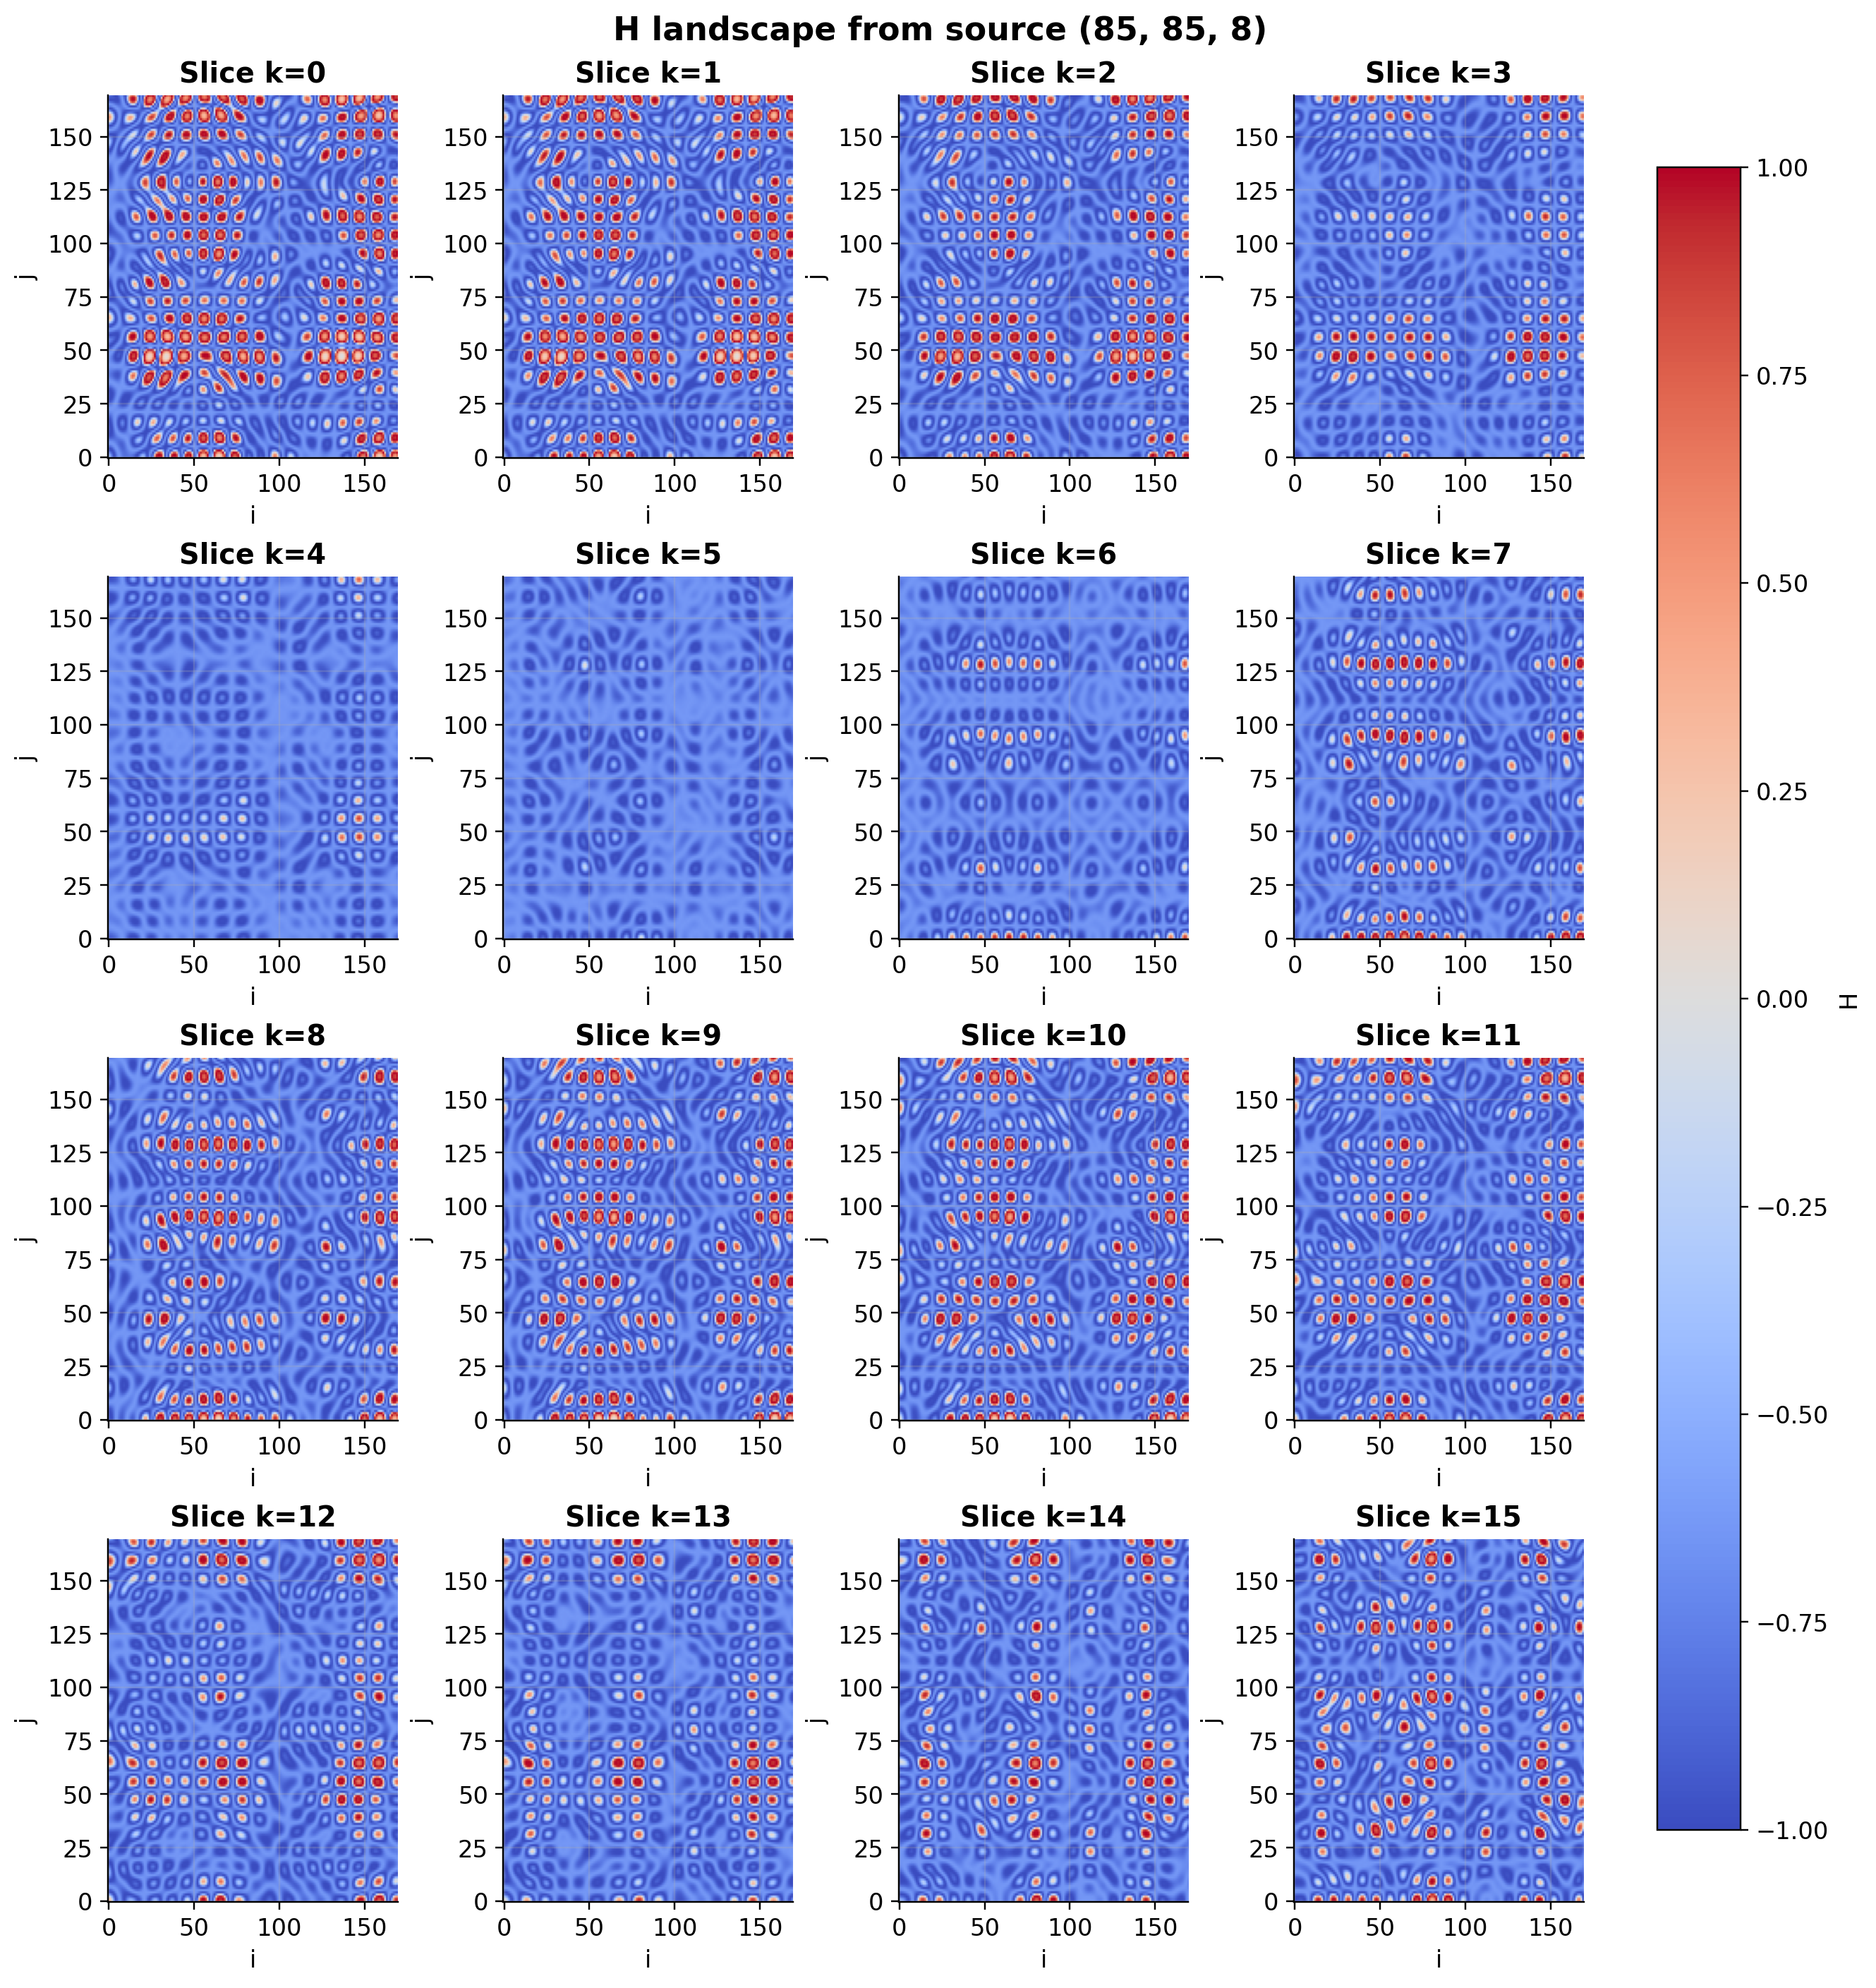
\includegraphics[width=0.98\linewidth,height=0.68\textheight,keepaspectratio]{generated_article_figures/extra_H_heatmaps.png}
		\caption{\footnotesize{Connection-affinity landscape $H_{85,85,8}(u,v,w,x)$ for one 64-digit connections gene on a $(170,170,16)$ tensor. Each panel corresponds to a target slice $w$, while the source and the common color range $[-1,1]$ remain fixed. These values are affinities, not an adjacency matrix of realized connections.}}
		\label{fig:affinity_H_slices}
	\end{figure}

	\begin{figure}[H]
		\centering
		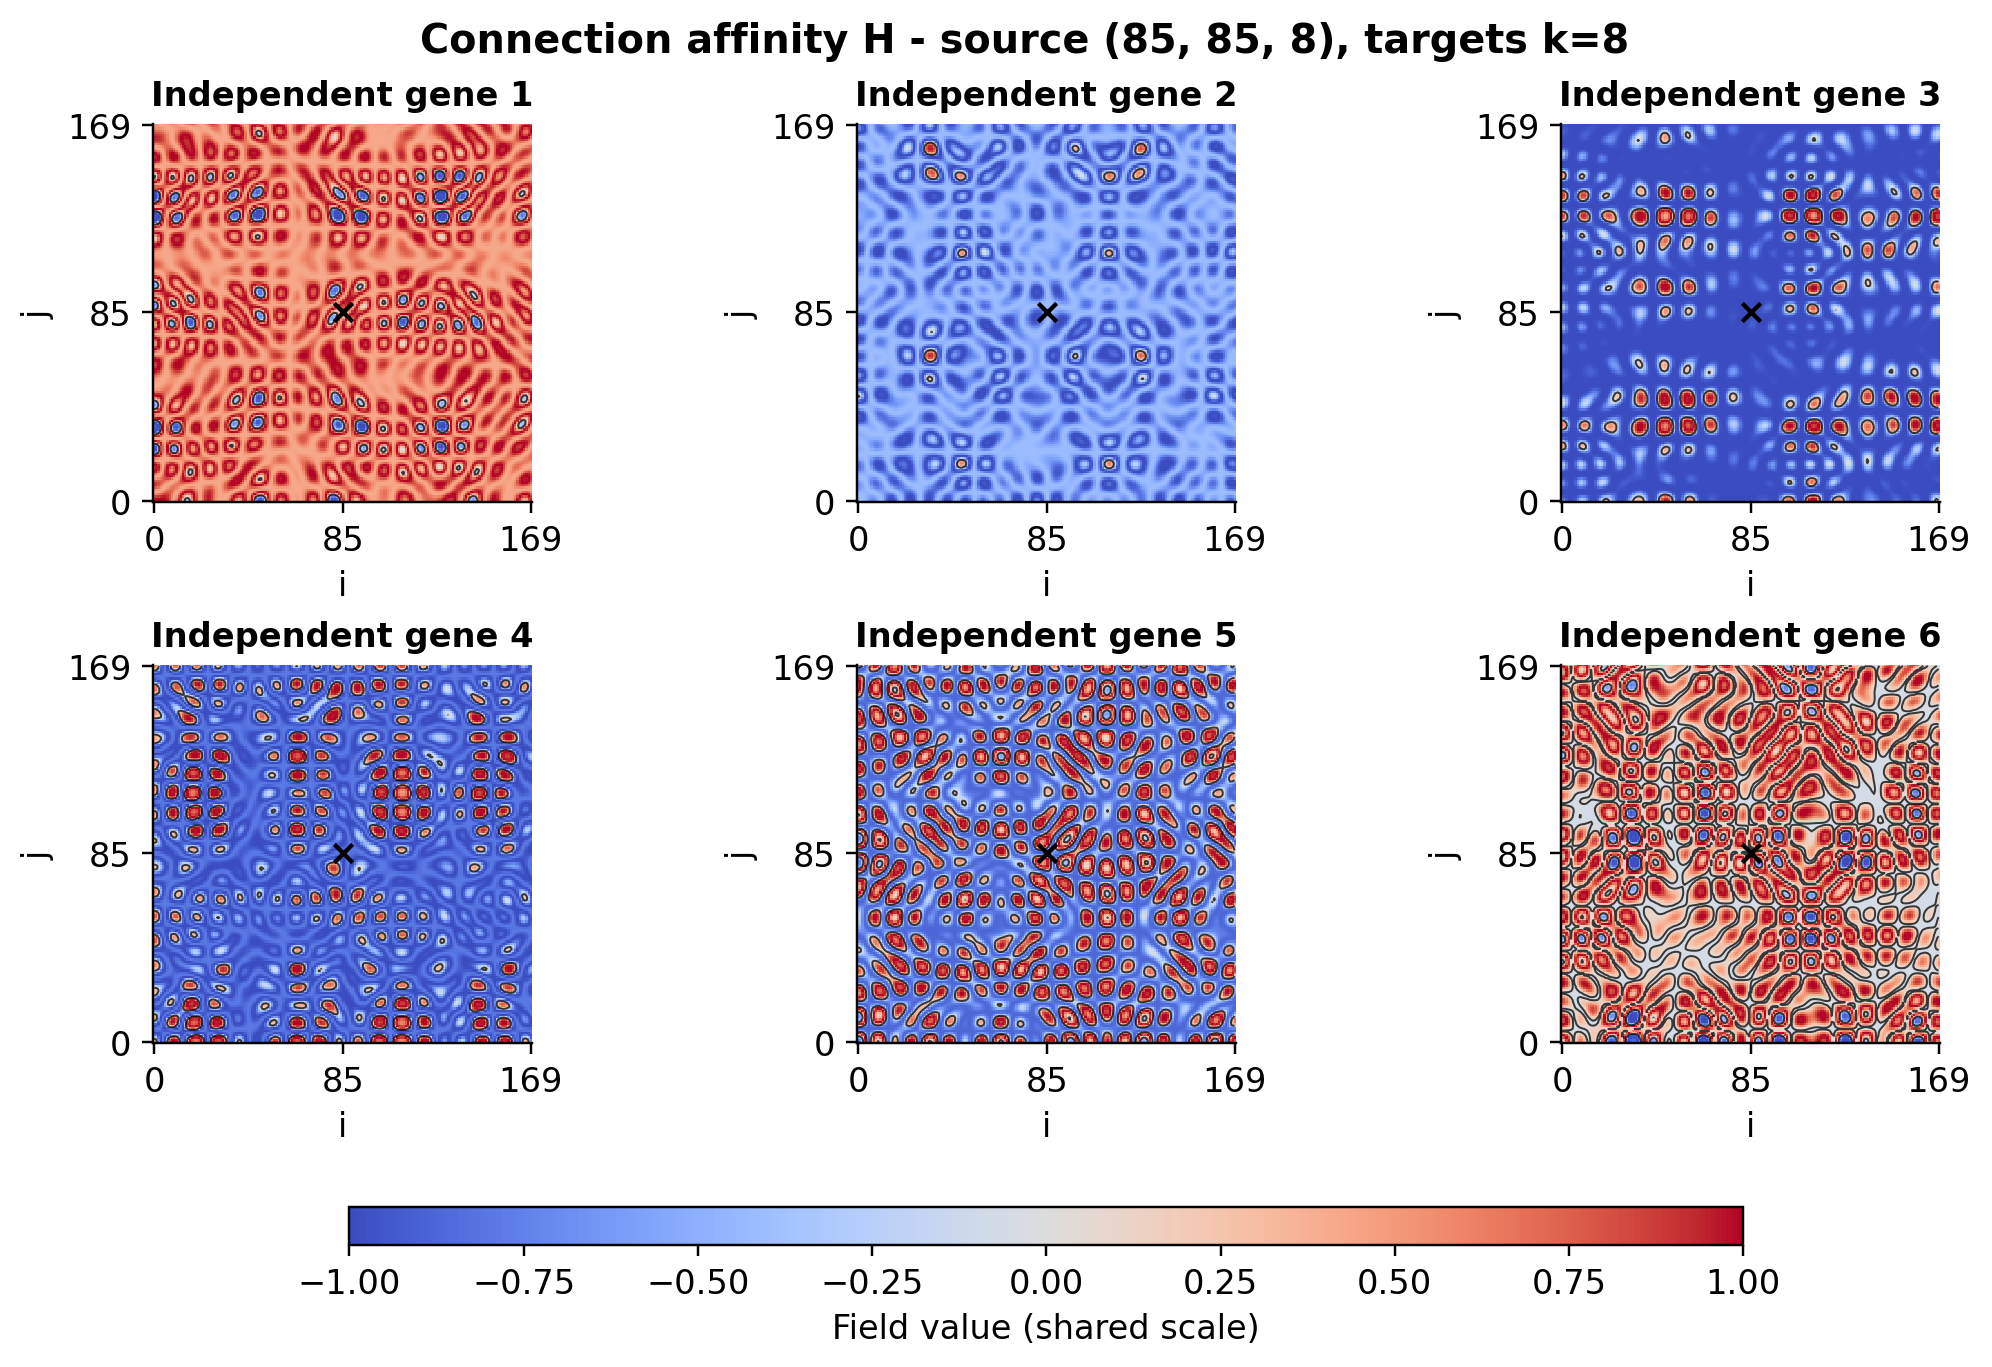
\includegraphics[width=0.98\linewidth,height=0.63\textheight,keepaspectratio]{generated_article_figures/extra_H_independent_genes_fixed_source.png}
		\caption{\footnotesize{Affinity in target slice $w=8$ for six independent 64-digit connections genes, with source $(85,85,8)$ fixed. Black contours, where present, mark the level $H=0$, the source itself is excluded as a candidate. All panels use the same color limits.}}
		\label{fig:affinity_H_genes}
	\end{figure}

	\begin{figure}[H]
		\centering
		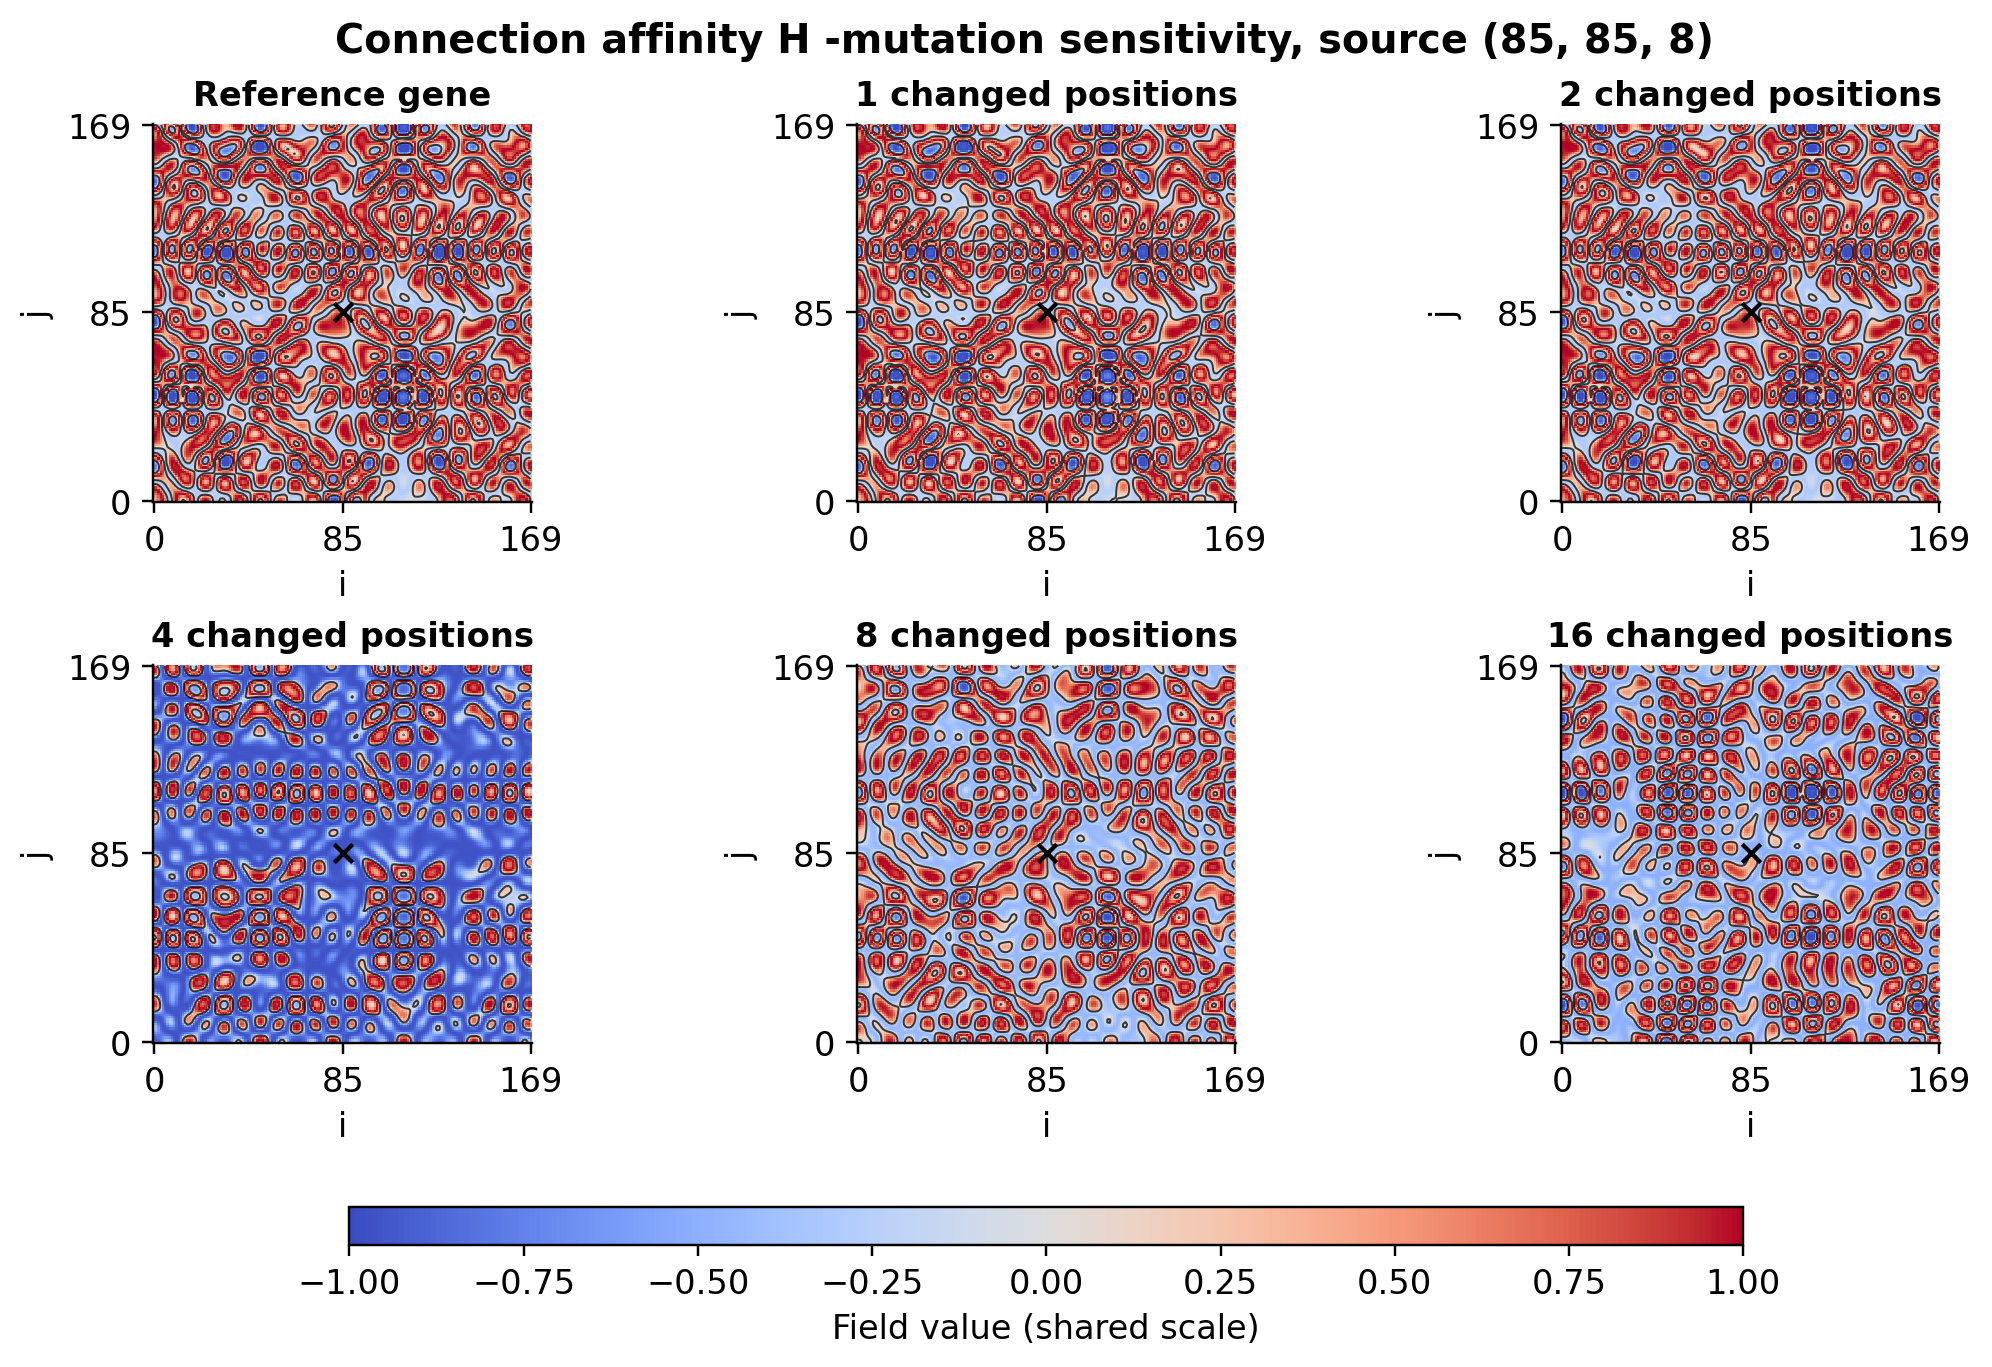
\includegraphics[width=0.98\linewidth,height=0.63\textheight,keepaspectratio]{generated_article_figures/extra_H_mutations_fixed_source.png}
		\caption{\footnotesize{Changes in $H$ after replacing exactly $1$, $2$, $4$, $8$, or $16$ digits of a reference 64-digit connections gene, with source $(85,85,8)$ and target slice $w=8$ fixed. Black contours, where present, indicate $H=0$, each gene defines both its own spatial field $A$ and its $H$ coefficients.}}
		\label{fig:affinity_H_mutations}
	\end{figure}

	Because $H$ depends on the source and target through their two scalar $A$ values, these visualizations should not be interpreted as evidence of arbitrary independent affinities between all pairs of neurons. They demonstrate structured variation within the particular genetic mapping defined above.
	
\section{Description}

We begin giving a list of items to describe our model of genetics and corresponding brain.

\begin{enumerate}			
	\item The maximum number $N_{max}$ of outgoing connections permitted for any neuron throughout its entire lifetime, including initial generation, developmental rescue, homeostatic reconnection, and structural plasticity, is a global value of the brain. It is defined by the gene $x = x_0 \ldots x_{7}$ through the formula

	$$N_{max}(x) = \max \left\{ 1, \ \lfloor \eta \cdot F_\beta(x) \rfloor \right\} = \max \left\{1, \left\lfloor \eta \cdot \sum_{t=0}^{7} \sqrt{1 + t} \cdot \beta^{x_t} \right\rfloor \right\}.$$
	
	The value $\eta > 0$ is an external parameter defined outside of the simulation. It is called the \emph{connections density}. The original model was design without this value (in other words, with $\eta = 1$), but later it was introduced so we can have a finer control over the overall amount of connections per neuron.

	\begin{figure}[H]
		\centering
		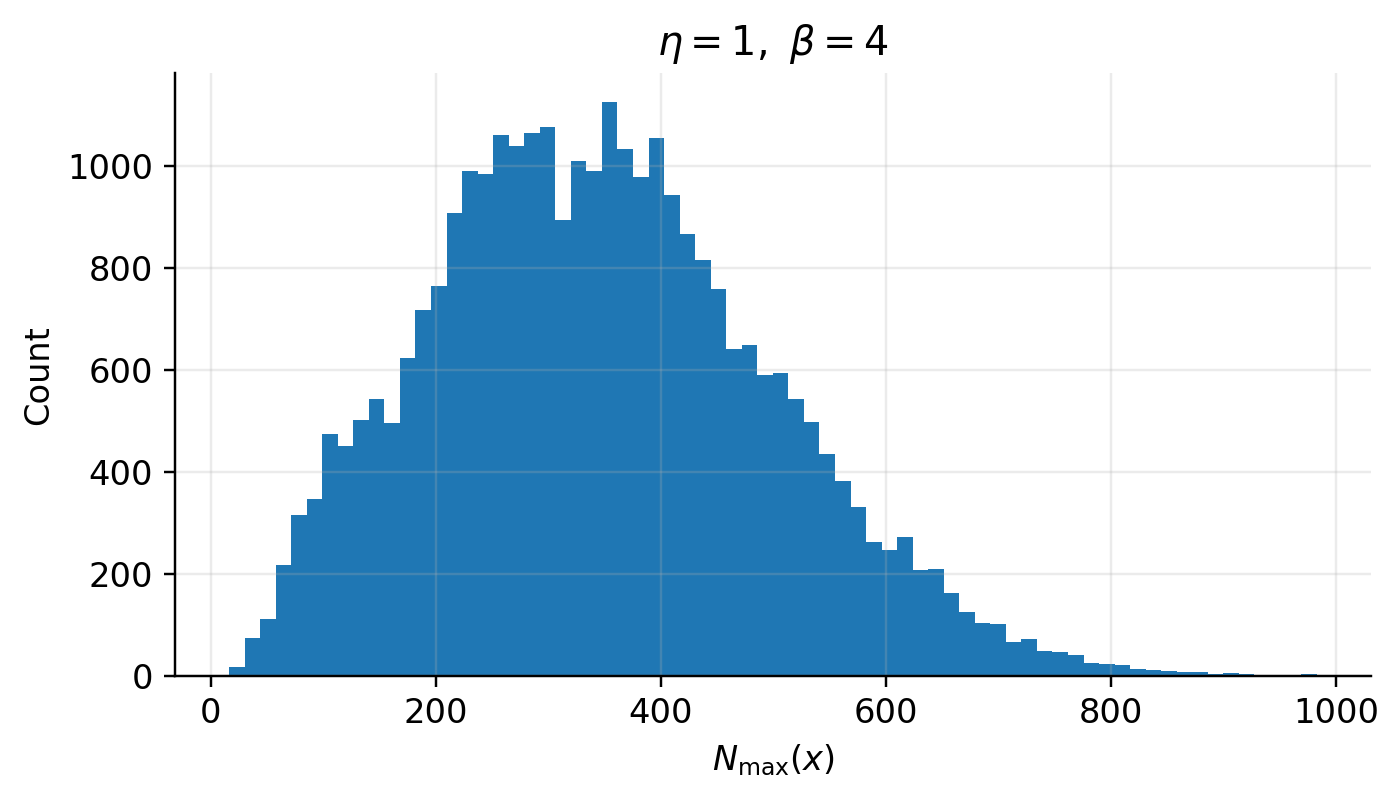
\includegraphics[width=0.80\linewidth,height=0.70\textheight,keepaspectratio]{generated_article_figures/Nmax_distribution.png}
		\caption{\footnotesize{Distribution of $N_{max}$ for $\eta = 1$ and $\beta = 4$. The horizontal axis shows the possible values of $N_{max}$, and the vertical axis gives their respective frequencies.}}
	\end{figure}

	This definition of $N_{max}$ depends on the value of $\beta$. Below, we show the highest value of $N_{max}$ for a few choices of $\beta$, with $\eta = 1$.

	\begin{center}
	\begin{tabular}{|c|c|}
		\hline
		$\beta$ & $\displaystyle{\max_x N_{max}(x)}$\\
		\hline
		1 & 16\\
		\hline
		2 & 130\\
		\hline
		4 & 1043\\
		\hline
		8 & 8348\\
		\hline
	\end{tabular}
	\end{center}

	For $\beta \geq 1$, the highest value of $N_{max}$ is approximately $16 \cdot \beta^3$. In practice, we want this maximum to be on the scale of $IJ$, meaning that the connection ceiling is comparable to approximately one entire slice. We therefore use $\sqrt[3]{IJ/16}$ as the reference scale for $\beta$.

	The value of $\beta$ is genetically determined. The gene $y = y_0 \ldots y_7$ defines $\beta$ through the formula

	$$\beta(y) = 1 + \frac{\displaystyle \sum_{t=0}^{7} \sqrt{1 + t} \cdot y_t}{3 \displaystyle \sum_{t=0}^{7} \sqrt{1 + t}} \cdot \sqrt[3]{\frac{IJ}{16}}.$$

	The fraction normalizes the weighted gene value to the interval $[0,1]$. Therefore, the gene $00000000$ produces $\beta = 1$, while $33333333$ produces the maximum value $\beta_{\max} = 1 + \sqrt[3]{IJ/16}$. Intermediate genes produce intermediate values of $\beta$, with the contribution of each position weighted by $W(t)=\sqrt{1+t}$. The resulting ceiling may be somewhat larger than $IJ$ at the upper end of the range, which is acceptable because $N_{max}$ is an upper bound on the number of simultaneously existing outgoing connections throughout the entire lifetime of each neuron, not a prescribed number of connections. When the bound is reached, further outgoing connections cannot be created until an existing connection dies and releases its slot. This makes the mapping from the gene to $\beta$ monotonic and directly interpretable.
	
	\item Let $n(i,j,k)$ denote the neuron at position $(i,j,k)$, with $0\leq i<I$, $0\leq j<J$, and $0\leq k<K$. The region of the initial search for connections is genetically determined. We introduce the \emph{initial search region gene} $y=y_0\ldots y_{63}$. Now let
	\begin{equation}
		S(y)=\frac{1-\sqrt{|\cos(G_{0,1}(y))|}}{10}.
		\label{initial_connection_extent}
	\end{equation}
	
	Since $|\cos(s)|\in[0,1]$, we have $S(y)\in[0,0.1]$. This coefficient determines the maximum search radius in each of the three spatial dimensions, relative to the corresponding tensor dimension.
	
	\begin{figure}[H]
		\centering
		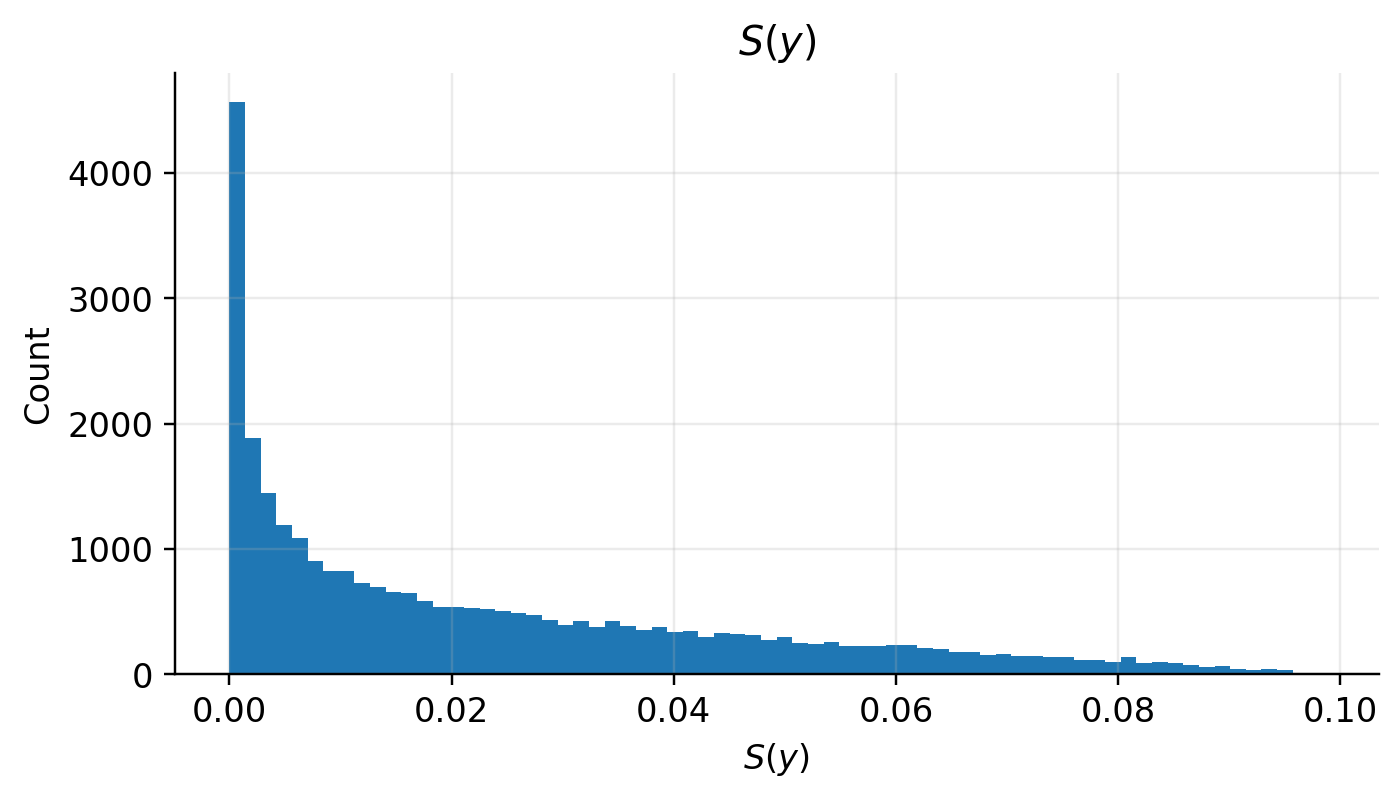
\includegraphics[width=0.80\linewidth,height=0.70\textheight,keepaspectratio]{generated_article_figures/S_distribution.png}
		\caption{\footnotesize{Distribution of $S(y)$. To generate the genes, each digit was drawn from the uniform distribution over $\{ 0, 1, 2, 3 \}$.}}
	\end{figure}
	
	For a source neuron $n(i,j,k)$, the set of candidate targets for the first pass of ordinary initial construction is
	\begin{equation}
	\begin{split}
	\mathcal{V}_{\mathrm{init}}(i,j,k,y)=\big\{(u,v,w):\;&0\leq u<I,\ 0\leq v<J,\ 0\leq w<K,\\
	&|u-i|\leq \lceil S(y) \cdot I\rceil,\\ 
	&|v-j|\leq \lceil S(y) \cdot J\rceil,\\
	&|w-k|\leq \lceil S(y) \cdot K\rceil,\quad (u,v,w)\neq(i,j,k)\big\}.
	\end{split}
	\label{initial_connection_neighborhood}
	\end{equation}
	
	Thus, the search covers a rectangular neighborhood centered at $n(i,j,k)$, truncated at the tensor boundaries. This rectangular restriction governs the first pass of the \emph{initial} connection search. It does not modify the spatial region available to structural plasticity during the brain's lifetime.

	\begin{figure}[H]
		\centering
		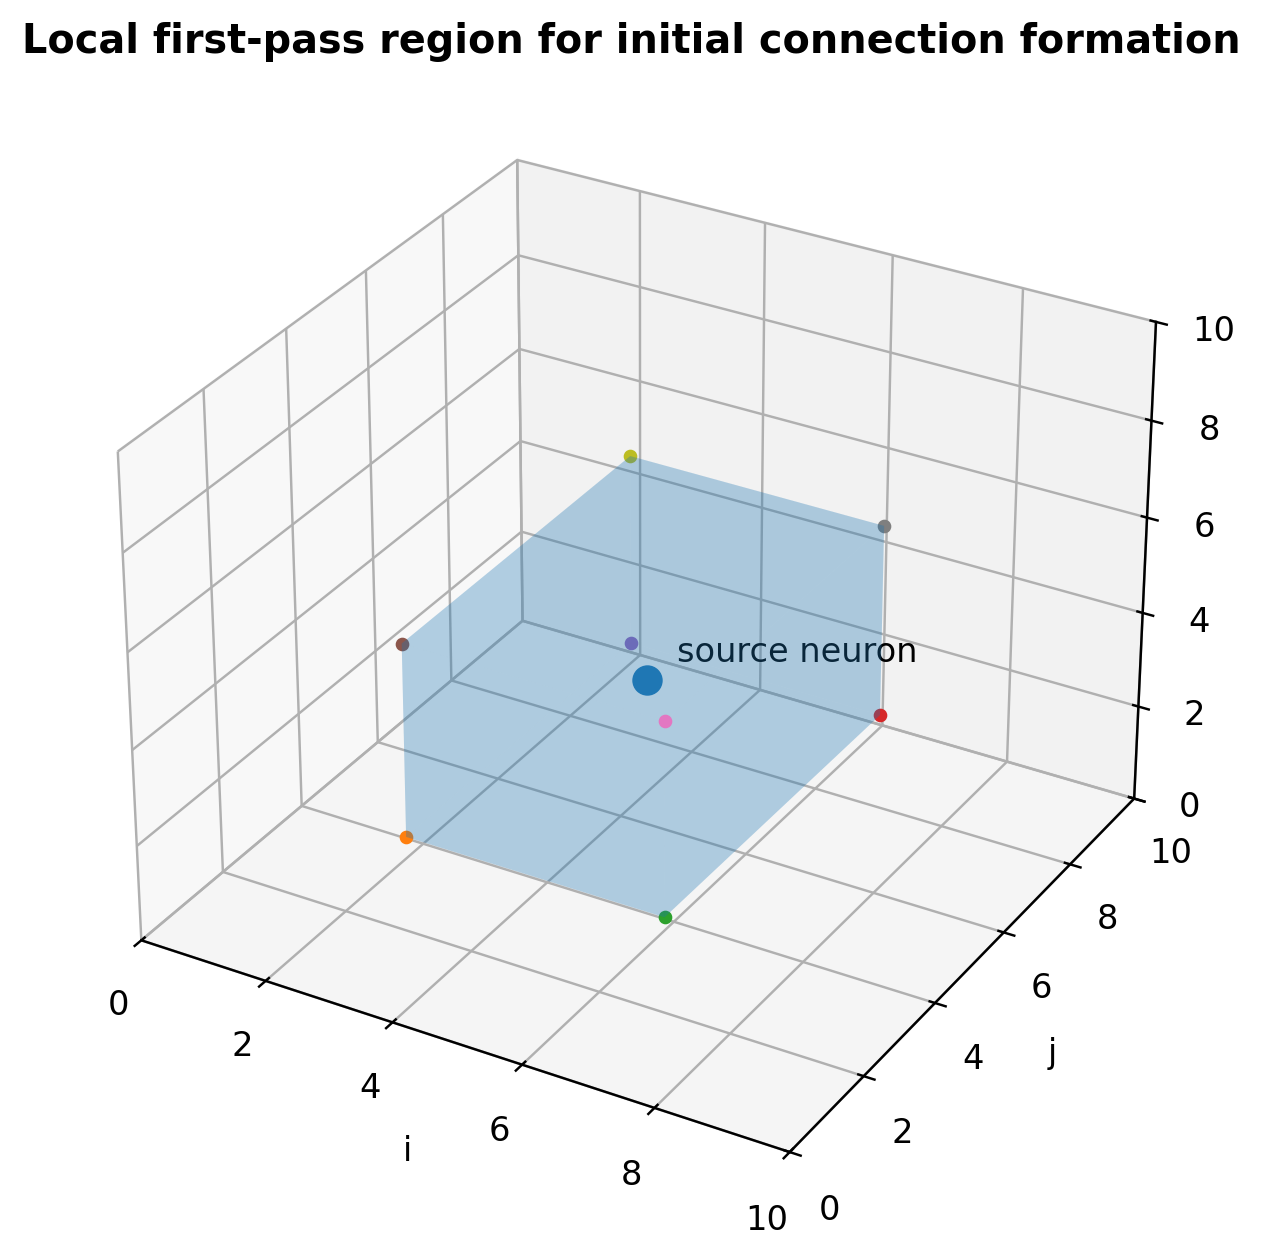
\includegraphics[width=0.73\linewidth,height=0.70\textheight,keepaspectratio]{generated_article_figures/connection_region.png}
		\caption{\footnotesize{Region of possible connections for a single neuron.}}
	\end{figure}

	\item The gene that determines the initial connections is a sequence of the form $x = x_0 \ldots x_{63}$, which we will call the \emph{connections gene}. For each neuron $n(i, j, k)$, a scalar activation field is evaluated for candidate targets in $\mathcal{V}_{\mathrm{init}}(i,j,k,y)$, where $y$ denotes the \emph{initial search region gene} defined above. For all neurons $n(u, v, w)$ in this region, we consider the value
	$$H_{i, j, k}(u, v, w, x).$$
	
	
	The associated values $A_{i, j, k}(x)$ in this context are called the \emph{connection energy} of $n(i, j, k)$, whereas $H_{i, j, k}(u, v, w, x)$ is the connection energy between $n(i, j, k)$ and $n(u, v, w)$.
	
	The two genes have distinct functions: $y$ specifies which targets are examined, whereas the connections gene $x$ determines the value of $H$ for each candidate. We consider that $n(i,j,k)$ and $n(u,v,w)$ are connected if 
	$$H_{i, j, k}(u, v, w, x) > 0.$$
	
	If more than $N_{max}$ candidates satisfy this condition, they are ordered by their values of $H$ and only the $N_{max}$ largest values are retained. Thus, $N_{max}$ acts as an upper bound on the outgoing degree during the initial generation of the brain rather than as a prescribed number of connections.

	The sign test can be visualized independently of the subsequent search and ranking steps:
	\begin{figure}[H]
		\centering
		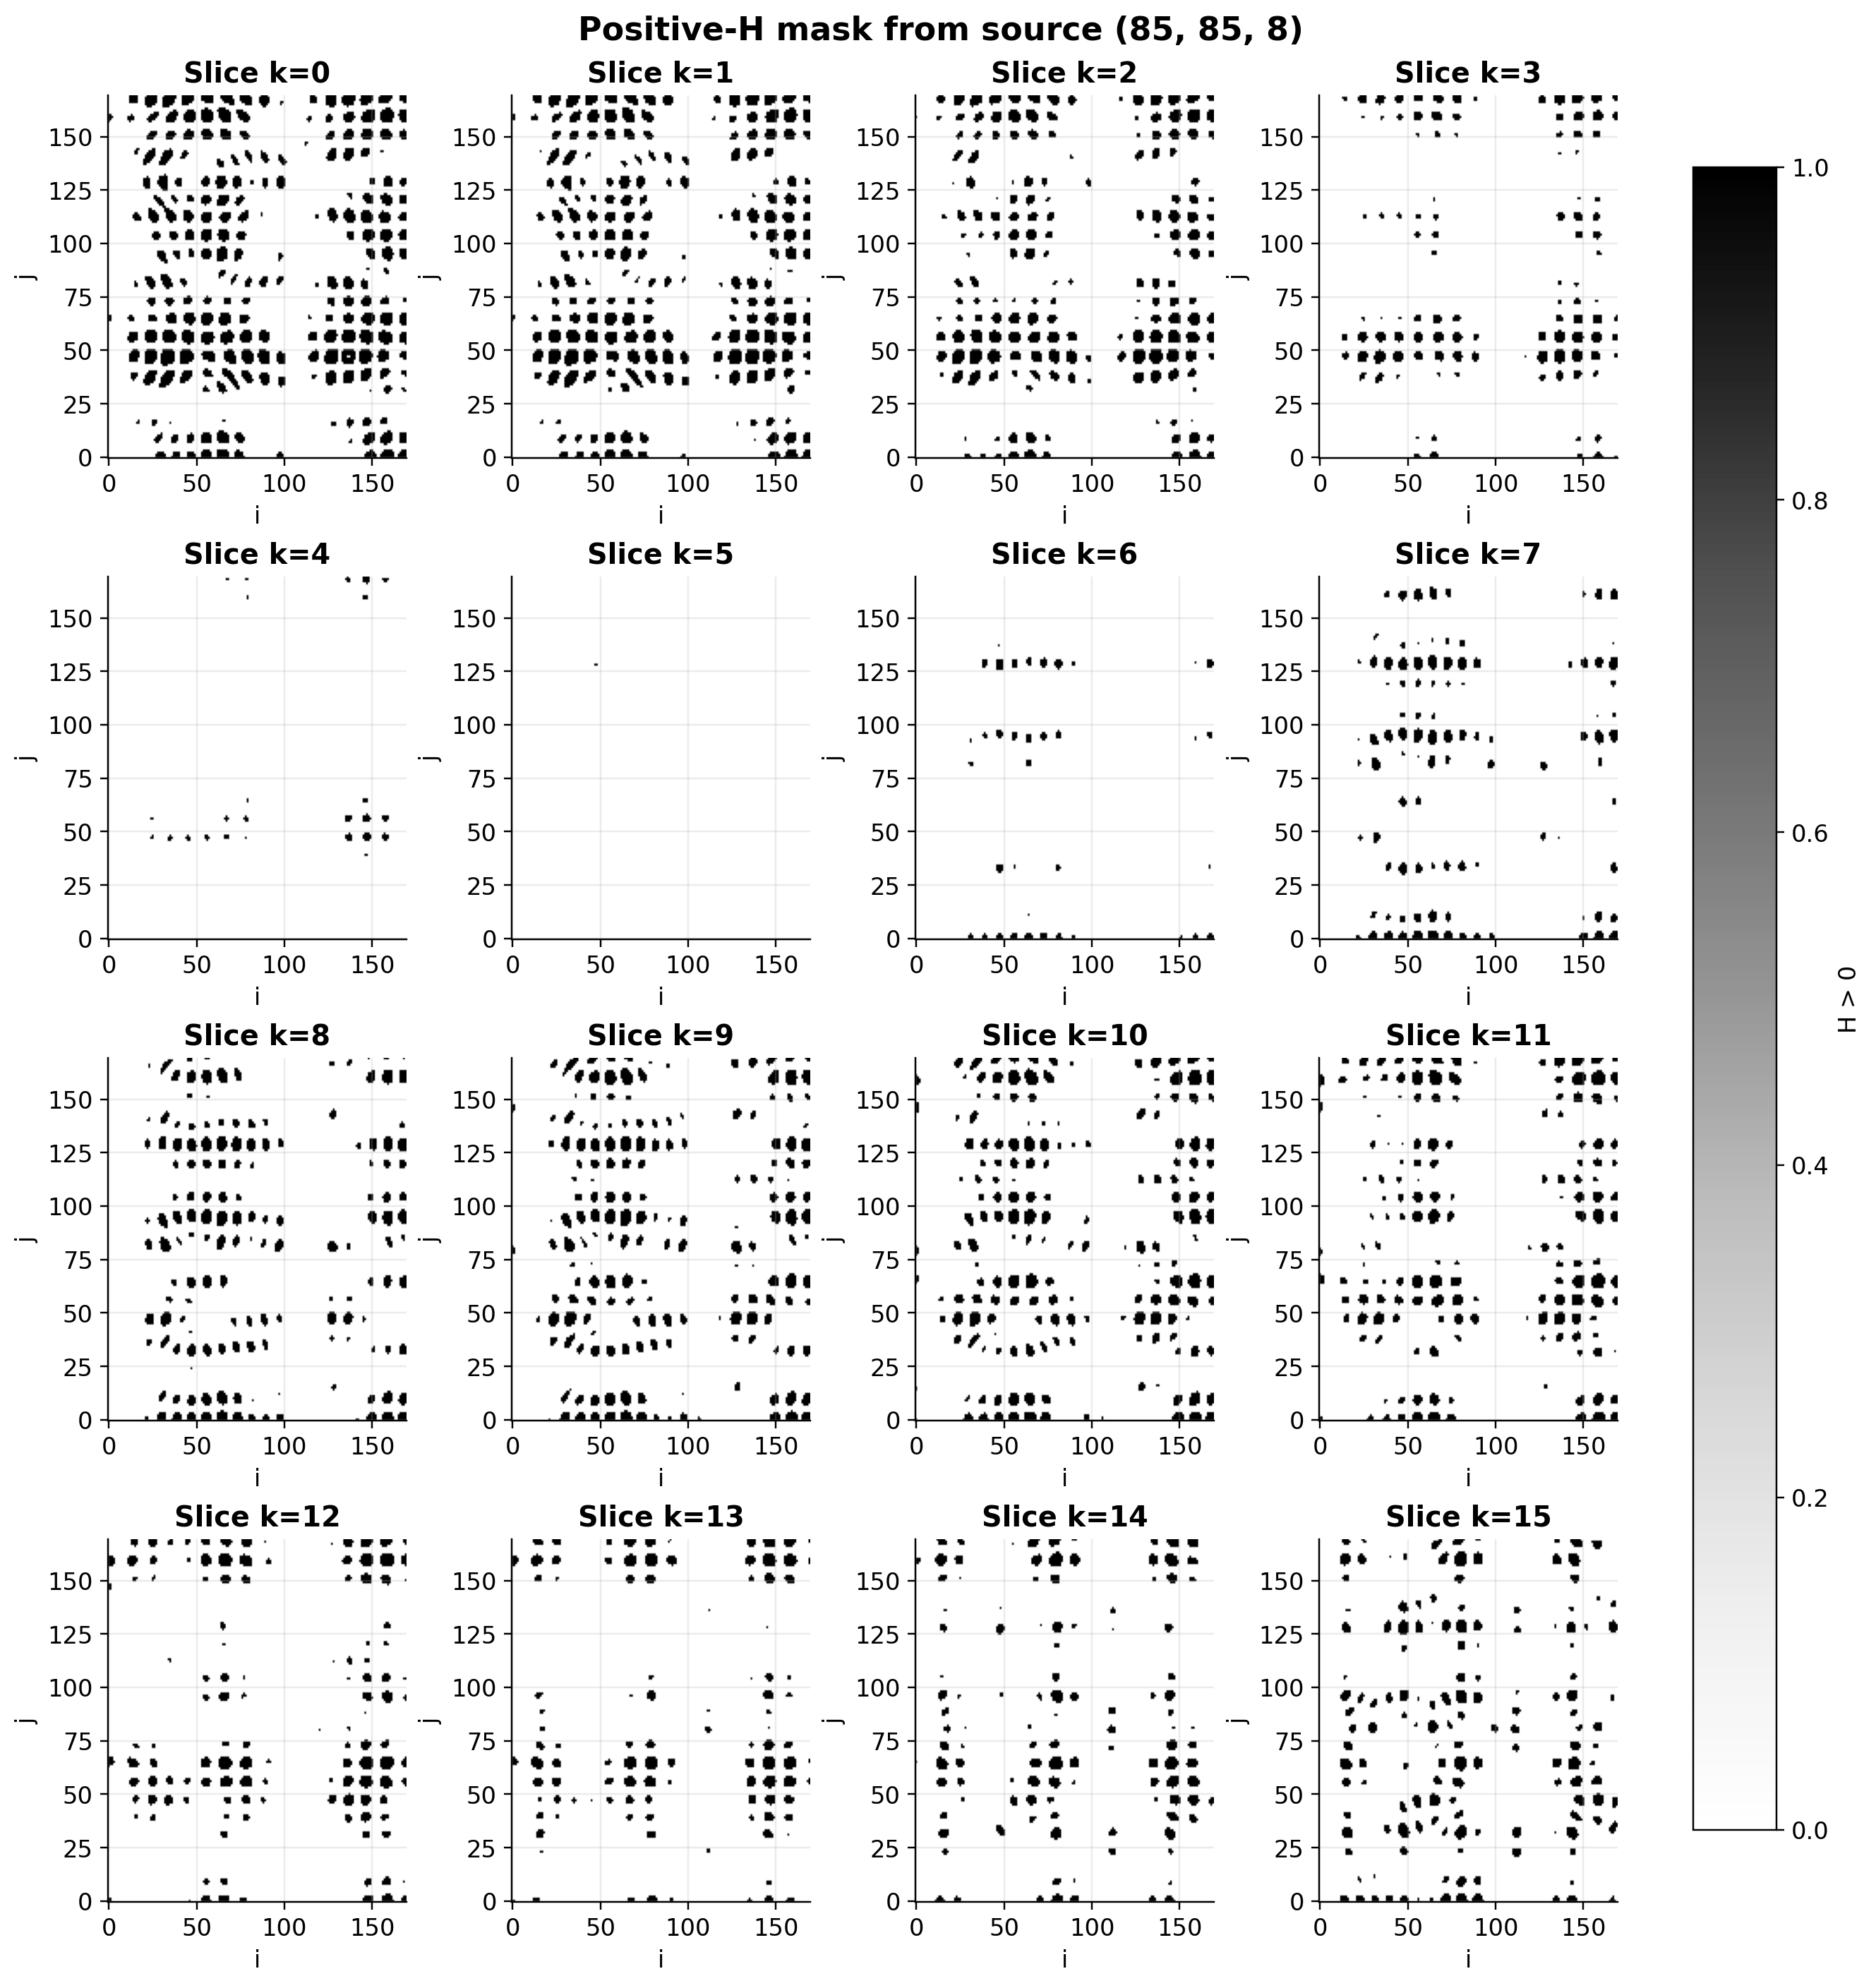
\includegraphics[width=0.98\linewidth,height=0.68\textheight,keepaspectratio]{generated_article_figures/extra_H_positive_mask.png}
		\caption{\footnotesize{Binary mask $\mathbf{1}_{\{H_{85,85,8}(u,v,w,x)>0\}}$ over all target slices for the same gene and source used in Figure~\ref{fig:affinity_H_slices}. Dark regions satisfy the positive-affinity condition. The mask does not account for the genetically restricted search region, self-connections, neuron-type restrictions, or the $N_{max}$ cap, therefore, dark pixels are eligible by sign, not necessarily actual synapses.}}
		\label{fig:affinity_H_positive_mask}
	\end{figure}

	\item If fewer than $N_{max}$ outgoing connections have been retained after this local pass, a second, bounded search for additional initial connections is performed. It uses the same initial search region gene $y=y_0\ldots y_{63}$, but examines targets outside the local neighborhood in Equation~\ref{initial_connection_neighborhood}. The search is deterministic and does not introduce any random choice.

	To construct candidate offsets, divide $y$ into three blocks $(y_0,\ldots,y_{20})$, $(y_{21},\ldots,y_{41})$, and $(y_{42},\ldots,y_{62})$. The final digit $y_{63}$ is not used in these offsets, but it still contributes to $S(y)$ through Equation~\ref{initial_connection_extent}. Let
	\begin{equation}
	\mathcal{Q}=\big\{(q_1,q_2,q_3,q_4):0\leq q_1<q_2<q_3<q_4<21\big\},
	\qquad |\mathcal{Q}|=\binom{21}{4}=5985.
	\label{additional_connection_combinations}
	\end{equation}
	
	Each ordered quadruple selects four positions in each block, retaining their relative order. The quadruples are visited in a fixed cyclic ordering. For $q\in\mathcal{Q}$, define the rotation
	\begin{equation}
	R_h(q)=\operatorname{sort}\!\left((q_1+h)\bmod21,\ldots,(q_4+h)\bmod21\right),
	\qquad h=0,\ldots,20.
	\label{additional_connection_rotation}
	\end{equation}
	
	The ordering begins with the 21 rotations of $(0,5,10,15)$, taken for $h=0,\ldots,20$. The remaining rotation orbits are visited by their lexicographically smallest representatives, in increasing lexicographic order, skipping the orbit already used. Within each orbit, the rotations are again visited for $h=0,\ldots,20$. Each orbit has 21 distinct quadruples, so the procedure visits all $5985$ quadruples exactly once. 

	Let $q^{(t)}=(q_{t,1},q_{t,2},q_{t,3},q_{t,4})$ be the quadruple at position $t$, starting with $t=0$. Form three four-digit \emph{decimal} numbers from the corresponding positions in the three blocks:
	\begin{equation}
	\begin{aligned}
	 s_t^{(i)}&=\sum_{\ell=1}^{4}10^{4-\ell}\,y_{q_{t,\ell}},\\
	 s_t^{(j)}&=\sum_{\ell=1}^{4}10^{4-\ell}\,y_{21+q_{t,\ell}},\\
	 s_t^{(k)}&=\sum_{\ell=1}^{4}10^{4-\ell}\,y_{42+q_{t,\ell}}.
	\end{aligned}
	\label{additional_connection_decimal_numbers}
	\end{equation}
	
	Leading zeros are allowed. For example, $0123$ represents the decimal number $123$. The unsigned offsets are then
	\begin{equation}
	(a_t,b_t,c_t)=\big(s_t^{(i)}\bmod I,\ s_t^{(j)}\bmod J,\ s_t^{(k)}\bmod K\big).
	\label{additional_connection_raw_offsets}
	\end{equation}

	The offsets are shifted so that the second pass examines only displacements outside the three-dimensional local neighborhood. Define
	\begin{equation}
	\begin{aligned}
	 r_i&=\lceil S(y)I\rceil, &D_i&=I-r_i-1,\\
	 r_j&=\lceil S(y)J\rceil, &D_j&=J-r_j-1,\\
	 r_k&=\lceil S(y)K\rceil, &D_k&=K-r_k-1.
	\end{aligned}
	\label{additional_connection_radii}
	\end{equation}

	For each axis with positive $D$, define a candidate displacement whose corresponding component necessarily exceeds the local search radius:
	\begin{equation}
	\begin{aligned}
	 d_t^{(i)}&=\big(r_i+1+(a_t\bmod D_i),\ b_t,\ c_t\big), &&D_i>0,\\
	 d_t^{(j)}&=\big(a_t,\ r_j+1+(b_t\bmod D_j),\ c_t\big), &&D_j>0,\\
	 d_t^{(k)}&=\big(a_t,\ b_t,\ r_k+1+(c_t\bmod D_k)\big), &&D_k>0.
	\end{aligned}
	\label{additional_connection_shifted_offsets}
	\end{equation}

	The preferred axis cycles through $i$, $j$, and $k$ according to $t\bmod 3$. If the displacement for that axis is unavailable because the corresponding $D$ is nonpositive, the next available axis in the same cyclic order is used. If all three are unavailable, no displacement can leave the local neighborhood while remaining within the dimensions of the tensor, and the second pass terminates. Denote the selected displacement by $d_t=(\widehat a_t,\widehat b_t,\widehat c_t)$. At least one of $\widehat a_t>r_i$, $\widehat b_t>r_j$, or $\widehat c_t>r_k$ holds, ensuring that every resulting valid target lies outside the neighborhood already searched. This construction allows the complementary search to reach any of the three dimensions rather than privileging only the first two.

	For each $d_t$, the eight signed displacements are examined in the following fixed order:
	\begin{equation}
	\begin{gathered}
	(+\widehat a_t,+\widehat b_t,+\widehat c_t),\quad(+\widehat a_t,+\widehat b_t,-\widehat c_t),\\
	(+\widehat a_t,-\widehat b_t,+\widehat c_t),\quad(+\widehat a_t,-\widehat b_t,-\widehat c_t),\\
	(-\widehat a_t,+\widehat b_t,+\widehat c_t),\quad(-\widehat a_t,+\widehat b_t,-\widehat c_t),\\
	(-\widehat a_t,-\widehat b_t,+\widehat c_t),\quad(-\widehat a_t,-\widehat b_t,-\widehat c_t).
	\end{gathered}
	\label{additional_connection_signs}
	\end{equation}
	
	A displacement is applied to the source position $(i,j,k)$. A new outgoing connection is created only if the resulting target is inside the tensor, is not the source itself, is not already connected to the source, and satisfies $H_{i,j,k}(u,v,w,x)>0$ for the \emph{connections gene} $x$. As in the first pass, the subsequent input/output restrictions still apply. No fixed bound of two slices is imposed on the initial connections: the depth displacement can reach any valid slice. Zero components or collisions after the modulo operations may produce repeated targets, these are simply rejected.

	The second pass stops as soon as the source has $N_{max}$ outgoing connections, after at most $N_{max}$ \emph{individual candidate tests}, or when the finite sequence of quadruples is exhausted, whichever occurs first. Each signed displacement tested counts toward this budget, including invalid and duplicate targets. Processing may therefore stop before all eight signs of a quadruple have been examined. Accepted connections are added in the prescribed order, without a further ranking pass. The maximum number of candidate tests in this second pass, over all neurons of one brain, is consequently $IJKN_{max}$, excluding the separate work of the local pass. This bounded search is part of initial construction and does not change the separately defined spatial rules for homeostatic reconnection and structural plasticity during the brain's lifetime.
	
	\item Each brain has a fixed number of neurons to receive inputs (external or internal signals supplied through the agent interface) and another fixed number of neurons to send outputs (actions on the environment or on the agent itself). Both of these numbers are determined outside the simulation. The input and output neurons form two distinct sets, that is, no neuron can be an input and output at the same time. 
	
	Let $\mathcal{N}_{in}$ be the set of neuron inputs, $\mathcal{N}_{out}$ be the set of neuron outputs, and $\mathcal{N}_{int}$ be the set of interior neurons (not input and not output). To assign these roles, let $x = x_0 \ldots x_{63}$ be the \emph{neuron role gene}. Then we define the \emph{neuron role map}

	\begin{equation}
	B_{i,j,k}(x)=\sin\!\left(4\pi A_{i,j,k}(x)\right).
	\label{role_order_score}
	\end{equation}
for each neuron $n(i, j, k)$.

	All $IJK$ neurons are ordered globally by increasing $B_{i,j,k}(x)$ (ties are resolved by spatial index). Following this order, the first $|\mathcal{N}_{in}|$ neurons with at least two outgoing connections are selected as inputs. Similarly, following the reverse order, the first $|\mathcal{N}_{out}|$ neurons with at least two incoming connections that have not already been selected as inputs are selected as outputs. All remaining neurons are internal. If either selection cannot provide the required number of neurons, brain construction is invalid and the brain is discarded.

	\item We require that input neurons send neural connections only to internal neurons and receive no neural connections from other neurons. Output neurons, conversely, receive neural connections only from internal neurons and do not send neural connections to other neurons. Thus, inputs and outputs can interact with the neural network only through internal neurons, and no direct input--input, input--output, or output--output connection is allowed.\footnote{Any input signal must be processed internally before reaching an output neuron.} Therefore, a subroutine is executed to clear any invalid connections. 	
	
	\item After the initial connections are created and invalid input/output connections are removed, some neurons may remain isolated with respect to the connectivity required by their role. Instead of immediately considering the brain invalid, a minimal \emph{developmental rescue} procedure is applied. Unlike ordinary initial connectivity, this exceptional procedure examines only the immediately adjacent neurons and uses the squared connection affinity $H^2$, allowing a strongly negative value of $H$ to be considered alongside a strongly positive one.

	For a neuron at $(i,j,k)$, let
	$$\mathcal{V}(i,j,k)=\left\{(u,v,w): |u-i|+|v-j|+|w-k|=1\right\},$$
	where only positions inside the brain tensor are retained. Thus, each neuron has at most six eligible spatial neighbors. The same orthogonal neighborhood is used later for the local modulatory field (Figure~\ref{fig:local_neighborhood}). Given a neuron $n$, let $\mathcal{I}(n)$ and $\mathcal{O}(n)$ denote its numbers of incoming and outgoing connections, respectively.

	\begin{itemize}
		\item For every internal or output neuron $n(u,v,w)$ such that $\mathcal{I}(n(u,v,w))=0$, candidate sources $n(i,j,k)$ are restricted to $\mathcal{V}(u,v,w)$. A candidate must satisfy
		$$H_{i,j,k}(u,v,w,x)^2>0$$
		and have available outgoing capacity under the strict lifetime limit,
		$$\mathcal{O}(n(i,j,k))<N_{\max}.$$
		If the isolated target is internal, its source may be either an internal or an input neuron, if the target is an output neuron, its source must be internal. Among all candidates satisfying these requirements, the source maximizing $H_{i,j,k}(u,v,w,x)^2$ is selected, and a new incoming connection is created.

		\item For every input neuron $n(i,j,k)$ such that $\mathcal{O}(n(i,j,k))=0$, candidate targets $n(u,v,w)$ are restricted to $\mathcal{V}(i,j,k)$ and must be internal neurons. Among those satisfying $H_{i,j,k}(u,v,w,x)^2>0$, the target maximizing $H_{i,j,k}(u,v,w,x)^2$ is selected, and a new outgoing connection is created. The input neuron remains subject to the same strict outgoing limit $N_{\max}$.
	\end{itemize}

	The initial weight of a rescued connection is obtained by applying the source-dependent attenuation to $H^2$ and enforcing the minimum initial weight of $0.1$, as specified in Equation~\ref{rescue_synaptic_weight} below. Consequently, no connection is created with zero initial weight. Only one connection is added for each neuron requiring rescue: one incoming connection for an isolated internal or output neuron, or one outgoing connection for an isolated input neuron. No existing connection is removed or redirected. If no neighboring candidate satisfies the positive-square condition, the input/output restrictions, and the strict outgoing capacity limit $N_{\max}$, brain construction fails and the brain is discarded.

	This rule preserves a genetic influence on the choice of the new connection without imposing the ordinary requirement $H>0$ on the emergency repair. Its search is local and limited to at most six neighboring positions, while the ordinary initial connectivity procedure first uses the genetically bounded region in Equation~\ref{initial_connection_neighborhood} and then, if needed, the additional candidate search defined above. The rescue does not guarantee that every initially isolated neuron can be connected, configurations without an admissible local candidate are still rejected.

	\item Consider that all initial neural connections have been established, including those added by developmental rescue. In the following expressions, $x$ denotes specifically the \emph{connections gene} used to compute $H$ and the corresponding connection field $A$, not the gene associated with any other neuronal parameter. Let $w_{i,j,k}^{u,v,w}\in[0,1]$ denote the weight of a directional connection from $n(i,j,k)$ to $n(u,v,w)$. For a connection established by the ordinary initial connectivity procedure, its weight, before enforcing the input-specific lower bound described later, is
	\begin{equation}
		w_{i,j,k}^{u,v,w}=\max\!\left\{\left(1-A_{i,j,k}(x)^2\right)H_{i,j,k}(u,v,w,x),\,0.1\right\}.
		\label{initial_synaptic_weight}
	\end{equation}

	For a connection created by \emph{developmental rescue}, the corresponding initial weight is instead
	\begin{equation}
		w_{i,j,k}^{u,v,w}=\max\!\left\{\left(1-A_{i,j,k}(x)^2\right)H_{i,j,k}(u,v,w,x)^2,\,0.1\right\}.
		\label{rescue_synaptic_weight}
	\end{equation}

	The source-dependent attenuation factor $1-A_{i,j,k}(x)^2$ is the same in both expressions. During ordinary construction, positive values of $H$ determine eligibility and ranking, during rescue, neighboring candidates are ranked by $H^2>0$, regardless of the sign of $H$. The attenuation and the minimum initial weight of $0.1$ are applied only after selecting the connection, so neither affects candidate ranking or eligibility. Thus, every connection created during initial development has weight in $[0.1,1]$, including cases where finite-precision evaluation of $A$ yields $|A|=1$ and the attenuation vanishes. This floor concerns the initial weight only, subsequent synaptic dynamics may weaken or remove connections. For connections originating from input neurons, the input-specific minimum weight defined below is also enforced using the \emph{input influence gene}, so their final initial weight is the maximum of the value in Equation~\ref{initial_synaptic_weight} or~\ref{rescue_synaptic_weight} (as appropriate) and $1/(1+\psi(x))$.

	\item All neurons always accept received signals and transmit them on\footnote{In the case the neuron is not an output neuron this is to send the signal to the other neurons. In the case the neuron is an output neuron, it will be actually converted into an action to be performed by the agent.}. Let $s \geq 0$ be this signal, this value is the sum of several signals coming from the connected neurons, and after the signal is transmitted the neuron signal is set to zero until a next signal is received. Then the neuronal signal to be transmitted on is given by
	$$1 - e^{-s/\kappa}.$$
	
	The function $\sigma(s) := 1 - e^{-s/\kappa}$ is called \emph{saturation function} and it is used to normalize signals. Here $\kappa \geq 1$ is the \emph{exponential factor} of the brain. It is a genetically defined parameter that controls how quickly a signal saturates. This value is determined by the formula
	$$\kappa(x) = F_{0.4}(x) = \sum_{t=0}^7 \sqrt{1 + t} \cdot 0.4^{x_t},$$
where  $x = x_0 \ldots x_7$ is the corresponding gene.

	We don't need $\kappa$ to assume high values, so the parameters in its formula are such that $\kappa$ is approximately in the interval $[1, 16]$. This is enough for our purposes.
	
	Note that the saturation function is the same for the entire brain.  
	
	\item Let $s = s_t(i, j, k)$ be the signal received by the neuron $n(i, j, k)$ at time $t$. Associated to each neuron there is a \emph{polarity factor} $\alpha \in \{-1, 1\}$ that defines the sign of the signal emitted by the neuron. Therefore, if the neuron $n(i, j, k)$ is allowed to emit its signal forward to $n(u, v, w)$, it will emit its weighed normalized signal with sign determined by its polarity factor. To be precise, it will emit the signal
	$$\alpha \cdot w_{i, j, k}^{u, v, w} \cdot \sigma(s).$$
	
	If $\alpha = 1$, we say the neuron is \emph{excitatory}, otherwise it is called \emph{inhibitory}. The polarity factor is defined by the gene $x = x_0 \ldots x_{63}$ through the formula
	$$\alpha_x(i, j, k) = 
		\left\{\begin{array}{ll}
			-1, & A_{i,j,k}(x) < A_{0,0,0}(x),\\
			1, & A_{i,j,k}(x) \geq A_{0,0,0}(x).
		\end{array}\right.$$
	
	Since inhibitory signals can decrease the state of their targets, the sum of the incoming signals may cause a provisional neuronal signal to become negative. However, neuronal signals are restricted to $s \geq 0$ throughout the simulation. Therefore, whenever an update would produce a negative signal, the lower bound is enforced by
	$$s_t(i,j,k) \leftarrow \max\left\{0, s_t(i,j,k)\right\}.$$
	In this way, inhibition can completely suppress neuronal activity, but it cannot produce negative neuronal signals.
	
	\item Input neurons are always excitatory. Therefore, every connection originating from an input neuron uses $\alpha=1$.
	
	\item Let $r$ be the raw signal received by an input neuron. 	The model does not prescribe how raw external information must be encoded. Each input channel applies an externally defined mapping $f$ that converts its raw input $r$, of arbitrary form, into a scalar $s = f(r) \in [0,1]$. This result is the actual signal received by the neuron. These transformations are external to the brain and they depend entirely of the agent we want to build. 
	
	The same goes to the outputs. After the final output is generated, it will be just a number. The subsequent action is a consequence of a function that determines what the agent should do based on the output number. These functions also are external to the brain. 
	
	When a simulation runs to generated the brain evolution, the brain itself is the "being"\ we want to fit in the set of inputs/outputs transformations previously designed. 
	
	\item Merely allowing input neurons to transmit external signals forward is not sufficient, because their signals compete in the postsynaptic sum with signals arriving from other neurons. To give evolution control over how strongly input signals influence the internal brain dynamics, we introduce an \emph{input influence gene}.

	Given a neuron $n$, define $\mathcal{I}(n)$ as the number of incoming connections to $n$ and $\mathcal{O}(n)$ as the number of outgoing connections from $n$. Let $x=x_0\ldots x_7$ be the input influence gene. After the initial brain generation, we define the input influence factor
	$$\psi(x) = \frac{1 + \sin\left(G_{1,1}(x)\right)}{|\mathcal{N}_{int}|} \sum_{n \in \mathcal{N}_{int}}\mathcal{I}(n).$$

	On average, an internal neuron has
	$$\frac{1}{|\mathcal{N}_{int}|} \sum_{n \in \mathcal{N}_{int}}\mathcal{I}(n)$$
incoming connections. This value is established during brain generation and remains fixed throughout the lifetime of the brain. Consequently, $\psi(x)$ is also fixed after generation and is not affected by connections subsequently created or removed by the lifetime dynamics.

	Let $s\in[0,1]$ be the state of the input neuron $n(i,j,k)$ at a certain moment. This state is transmitted forward as the amplified signal $\psi(x)s$, allowing the input signal to compete with the aggregate activity received from other neurons. The normalization $\sigma$ is not applied to the transmitted input signal, avoiding an unnecessary loss of information before this amplification. Since input neurons are excitatory by definition, the signal transmitted through an existing connection to an internal neuron $n(u,v,w)$ is
	$$w_{i,j,k}^{u,v,w} \cdot \psi(x) \cdot s.$$

	The factor $1+\sin\left(G_{1,1}(x)\right)\in[0,2]$ controls how strongly the initial mean incoming degree contributes to the amplification of input signals. Its distribution is given below.

	\begin{figure}[H]
		\centering
		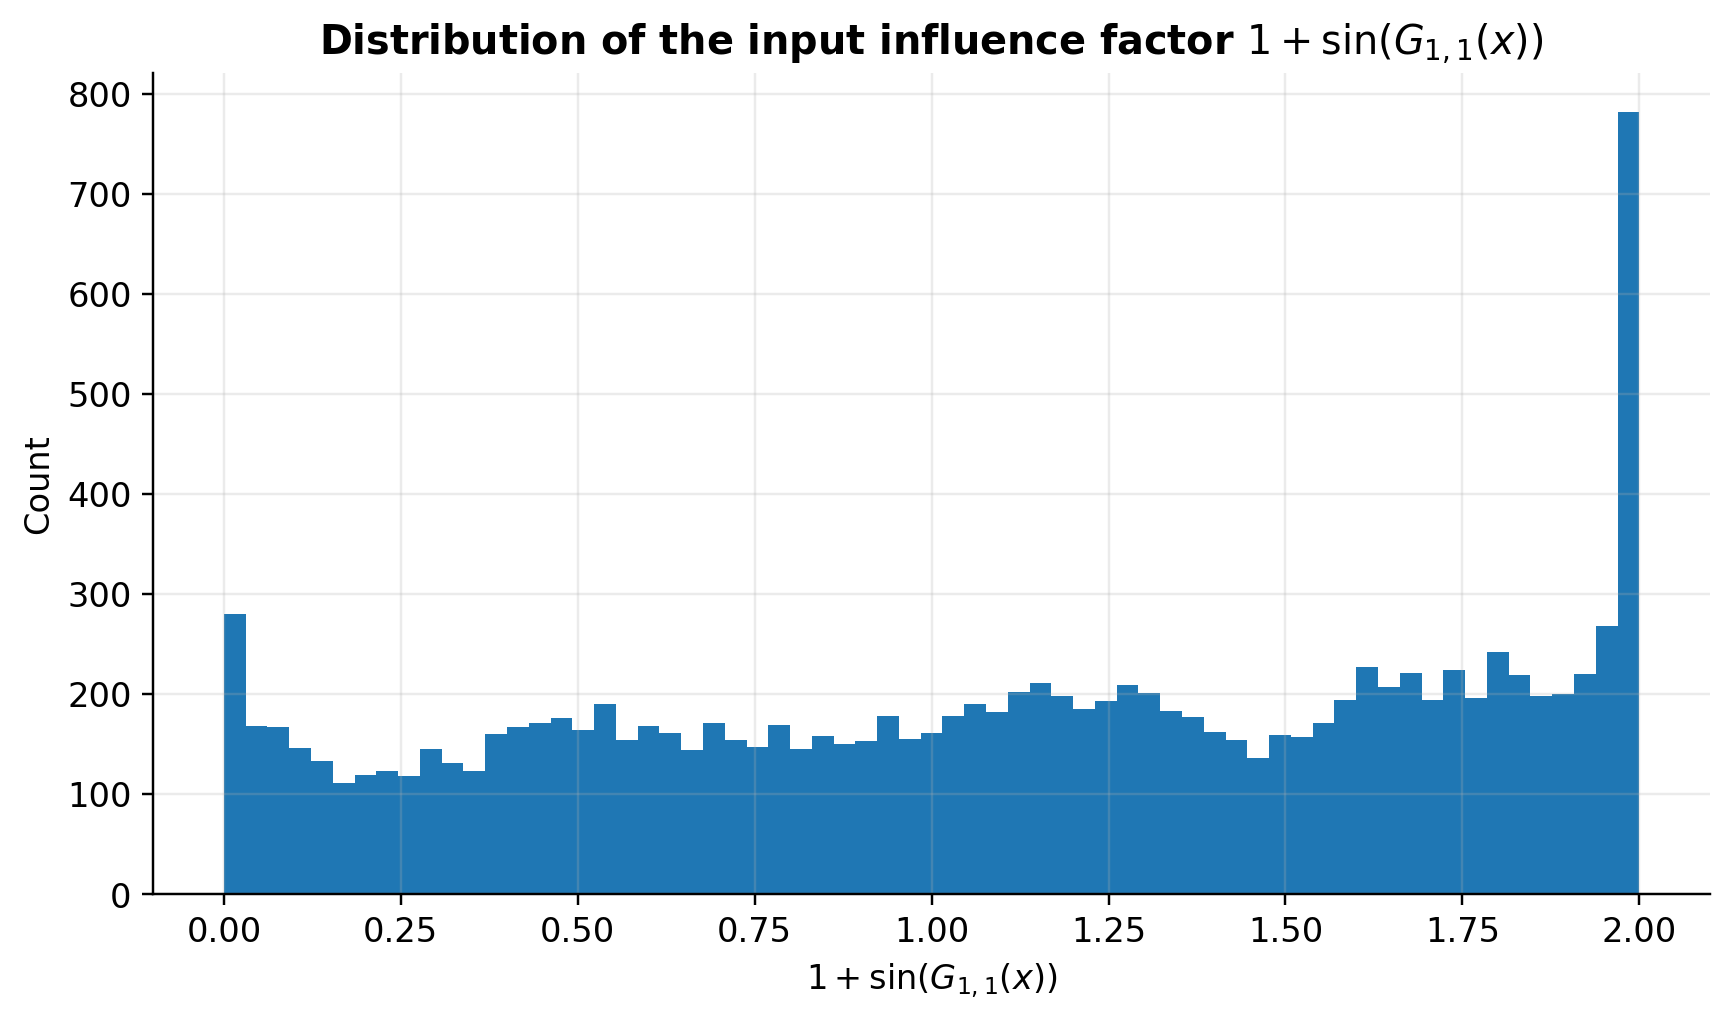
\includegraphics[width=0.83\linewidth,height=0.70\textheight,keepaspectratio]{generated_article_figures/input_influence_distribution.png}
		\caption{\footnotesize{Distribution of the input influence factors $1+\sin\left(G_{1,1}(x)\right)$. To generate the genes, each digit was drawn from the uniform distribution over $\{0,1,2,3\}$.}}
	\end{figure}

    \item Connections originating from input neurons are preserved throughout the lifetime of the brain. They do not undergo passive synaptic decay. To prevent these connections from becoming functionally negligible, their weights are constrained by
	$$\frac{1}{1+\psi(x)}\leq w_{i,j,k}^{u,v,w}\leq1.$$
	
	After each synaptic update, this interval is enforced by
	$$w_{i,j,k}^{u,v,w}\leftarrow \max \left\{ w_{i,j,k}^{u,v,w},\frac{1}{1+\psi(x)} \right\}.$$
	
	The lower bound depends on the genetically determined input influence itself. If $\psi(x)=0$, the weight is forced to $1$, but the transmitted input signal remains zero.
	
\end{enumerate}

\subsection{Synchronous neuronal update}
Let $\operatorname{Pred}_{int}(i)$ and $\operatorname{Pred}_{in}(i)$ denote the internal and input sources of a non-input neuron $i$, respectively. The actual update during one discrete simulation iteration is
\begin{equation}
\boxed{\displaystyle
s_i(t+1)=\max\!\left\{0,\sum_{j\in\operatorname{Pred}_{int}(i)}\alpha_j w_{ji}\sigma\big(s_j(t)\big)
+\sum_{j\in\operatorname{Pred}_{in}(i)}w_{ji}\psi\,s_j^{\mathrm{in}}(t)\right\}.}
\label{simple_discrete_update}
\end{equation}
The second sum is empty for output neurons. Inputs have no neural predecessors, and their states are externally refreshed rather than computed by this equation. All source values at time $t$ are read from the same time slice before any next state is committed; hence a signal traverses at most one directed connection per iteration. In particular, $s_i(t)$ is \emph{not} added to $s_i(t+1)$. After emission the previous state is discarded. An output signal exposed to the agent at iteration $t$ is $o_i(t)=\sigma(s_i(t))$. Recurrent synaptic loops may preserve patterns of activity across iterations despite this absence of single-neuron retention. No additional external term enters the internal-neuron equation.

\section{Overview}
The parameters selected outside the evolving genome are the brain dimensions $(I,J,K)$, connection-density parameter $\eta$, and input and output channel counts. The simplified genome contains exactly eight genes:
\begin{table}[H]\centering\small
\begin{tabular}{p{9cm}rc}\toprule
\textbf{Feature} & \textbf{Digits} & \textbf{Scope} \\\midrule
Maximum outgoing degree $N_{max}$ & 8 & Global \\
Base $\beta$ for the outgoing degree ceiling & 8 & Global \\
Initial connection search region & 64 & Global \\
Initial connection affinities and weights & 64 & Spatial \\
Neuron input/output role map & 64 & Spatial \\
Exponential factor $\kappa$ & 8 & Global \\
Excitatory/inhibitory polarity & 64 & Spatial \\
Input influence $\psi$ & 8 & Global \\\bottomrule
\end{tabular}
\caption{Genetic parameters of the Vsimple model. Spatial features are evaluated at neuron coordinates.}
\label{model_gens}
\end{table}
There are $288$ base-four digits, corresponding to $4^{288}\approx10^{173}$ possible genomes. The synaptic graph, weights, polarity, input influence, and saturation parameter are determined during construction, and then remain immutable for the individual's lifetime.

\section{Evolutionary Selection of Fixed Networks}
No synaptic reinforcement, synaptic decay, eligibility traces, endogenous modulatory field, homeostatic correction, or structural plasticity is performed during individual execution. Consequently, any change in the weights or connectivity of a descendant must come from producing a new genome and constructing its new brain, not from plasticity in the parent.

Evolutionary selection may favor brains whose initial connectivity, fixed weights, polarities, input sensitivity, and recurrent dynamics generate useful agent behavior. A recurrent fixed-weight network can respond differently to the same current input depending on internal states left by preceding inputs. Such memory is a property of network-level recurrent activity, not persistence of the state of a single neuron or changes in synapses. Evolutionary success on a specific environment does not, by itself, demonstrate general learning or adaptation through synaptic change.

\section{Inputs and Outputs}
Inputs and outputs are general interfaces between the brain and its agent. Inputs may encode sensory observations or internally accessible agent variables, but the \emph{only} entry points to the neural network are the designated input neurons. No direct external stimulation term is added to internal or output neurons. Inputs are always excitatory, emit $w\psi s^{\mathrm{in}}$ through their fixed outgoing connections, and receive no neural edges. Output neurons receive only internal connections and have no outgoing neural edges. At each step, an output exposes $\sigma(s)$ to the external action mapping. A closed feedback loop through the environment or an observable agent variable is possible only through these explicitly defined input and output interfaces.

\section{Offspring}
Let $X=(x^{(1)},\ldots,x^{(8)})$ and $Y=(y^{(1)},\ldots,y^{(8)})$ denote two homologous eight-gene genomes. Reproduction follows the same genetic method as the earlier model:
\begin{enumerate}
\item Only homologous genes undergo crossover.
\item Each 8- or 64-digit gene is partitioned into successive blocks of four digits. Each child block is independently copied from the corresponding block of either parent with probability $1/2$.
\item Each digit is then independently considered for mutation with a configurable probability (default $p_{mut}=0.001$). A selected digit is replaced by a value sampled uniformly from $\{0,1,2,3\}$. A mutation may sample the original value.
\end{enumerate}
An offspring brain is built afresh from its resulting genome. It does not inherit mutable neural states from either parent.

\section{Memory Consumption}
Let $N=IJK$ and $E=N\,N_{max}$ be the number of neurons and reserved outgoing slots of a brain. In the present Vsimple GPU implementation, the original V9 neuron buffer layout and fixed-slot synapse representation are retained for compatibility with existing visualization and construction tools. During construction, temporary GPU buffers contain the candidate connections and adjacency-building data. Once the graph is finalized, a receiver-indexed compressed sparse row (CSR) lookup is built once and the construction scratch buffers are released.

The resident runtime allocation per brain uses 32 bytes per neuron for phenotype data, 4 for role, 48 for state/visualization data, 4 for accumulated incoming signal, 4 for source emission, 4 each for outgoing count, outgoing degree, incoming degree, CSR offset, CSR length, input reverse map, and output reverse map. Together these are $120N$ bytes. Reserved connection slots occupy $16E$ bytes and CSR edge indices another $4E$ bytes. Thus the approximate GPU runtime allocation per brain is
\begin{equation}
\boxed{\operatorname{Mem}_{\mathrm{Vsimple}}\approx120N+20E\quad\text{bytes}}
\label{simple_memory}
\end{equation}
plus fixed per-agent parameter blocks, input/output streams, driver allocation overhead and optional visualization/inspection buffers. This is a description of the current conservative buffer layout, not a theoretical minimum. In particular, fixed weights and topology make the per-synapse eligibility state and all synaptic-update buffers unnecessary. The fixed $N_{max}$ slot capacity can still dominate memory even if many slots remain empty. Multiple brains are stored in disjoint segments of the same GPU buffers.

\section{Compute Shaders}
The Vsimple execution keeps the original Godot/RenderingDevice compute-shader architecture and the existing visualization framework. Build-time stages evaluate spatial gene fields, choose the initial connectivity, assign neuron roles, remove invalid edges, perform developmental rescue, and finalize fixed synaptic weights. The fixed outgoing slots are then converted into a receiver-indexed CSR lookup once. During an individual's lifetime, neither the edge buffer nor the CSR index is modified.

A synchronous neural step is implemented with three main GPU compute stages:
\begin{enumerate}
\item \textbf{Prepare emissions:} read each current neuronal state; for an input source, read only its assigned external input channel and compute $\psi s^{\mathrm{in}}$; for an internal source, compute $\alpha\sigma(s)$. All source emissions for iteration $t$ are completed before propagation.
\item \textbf{Sparse propagation:} for each non-input target, traverse its incoming CSR row and accumulate $w_{ji}$ times the emission of each source $j$. This is a sparse matrix--vector operation with fixed weights; no synaptic update is performed.
\item \textbf{Advance state:} write the new state as $\max(0,\text{incoming sum})$ (or zero for an input, whose next sample will come from the interface), expose the \emph{current} normalized output activity $\sigma(s_i(t))$ to the agent, and discard the preceding neuron state.
\end{enumerate}

The compute-shader execution uses barriers between stages so every source emission is available before accumulation and every output is computed before overwriting the state. When the agent or a simulation restarts a brain, only neural activity buffers are cleared; the fixed connectivity, weights and CSR lookup remain intact. This eliminates lifetime Hebbian updates, decay, structural changes, refractory handling, retention, modulatory-field propagation, eligibility updates, and CSR rebuilding. The theoretical complexity of each neural step is $O(N+E_{\mathrm{active}})$, excluding host-to-GPU input transfers, GPU-to-host output readback, and device synchronization.

\end{document}

